%% RiSE Latex Template - version 0.5
%%
%% RiSE's latex template for thesis and dissertations
%% http://risetemplate.sourceforge.net
%%
%% (c) 2012 Yguaratã Cerqueira Cavalcanti (yguarata@gmail.com)
%%          Vinicius Cardoso Garcia (vinicius.garcia@gmail.com)
%%
%% This document was initially based on UFPEThesis template, from Paulo Gustavo
%% S. Fonseca.
%%
%% ACKNOWLEDGEMENTS
%%
%% We would like to thanks the RiSE's researchers community, the 
%% students from Federal University of Pernambuco, and other users that have
%% been contributing to this projects with comments and patches.
%%
%% GENERAL INSTRUCTIONS
%%
%% We strongly recommend you to compile your documents using pdflatex command.
%% It is also recommend use the texlipse plugin for Eclipse to edit your documents.
%%
%% Options for \documentclass command:
%%         * Idiom
%%           pt   - Portguese (default)
%%           en   - English
%%
%%         * Text type
%%           bsc  - B.Sc. Thesis
%%           msc  - M.Sc. Thesis (default)
%%           qual - PHD qualification (not tested yet)
%%           prop - PHD proposal (not tested yet)
%%           phd  - PHD thesis
%%
%%         * Media
%%           scr  - to eletronic version (PDF) / see the users guide
%%
%%         * Pagination
%%           oneside - unique face press
%%           twoside - two faces press
%%
%%		   * Line spacing
%%           singlespacing  - the same as using \linespread{1}
%%           onehalfspacing - the same as using \linespread{1.3}
%%           doublespacing  - the same as using \linespread{1.6}
%%
%% Reference commands. Use the following commands to make references in your
%% text:
%%          \figref  -- for Figure reference
%%          \tabref  -- for Table reference
%%          \eqnref  -- for equation reference
%%          \chapref -- for chapter reference
%%          \secref  -- for section reference
%%          \appref  -- for appendix reference
%%          \axiref  -- for axiom reference
%%          \conjref -- for conjecture reference
%%          \defref  -- for definition reference
%%          \lemref  -- for lemma reference
%%          \theoref -- for theorem reference
%%          \corref  -- for corollary reference
%%          \propref -- for proprosition reference
%%          \pgref   -- for page reference
%%
%%          Example: See \chapref{chap:introduction}. It will produce 
%%                   'See Chapter 1', in case of English language.

\documentclass[en,twoside,onehalfspacing]{risethesis}

\usepackage[english]{babel}
\usepackage{colortbl}
\usepackage{color}
\usepackage[table]{xcolor}
\usepackage{microtype}
\usepackage{bibentry}
\usepackage{subfigure}
\usepackage{multirow}
\usepackage{rotating}
\usepackage{booktabs}
\usepackage{pdfpages}
\usepackage{caption}
\usepackage{lipsum}

\captionsetup[table]{position=top,justification=centering,width=.85\textwidth,labelfont=bf,font=small}
\captionsetup[lstlisting]{position=top,justification=centering,width=.85\textwidth,labelfont=bf,font=small}
\captionsetup[figure]{position=bottom,justification=centering,width=.85\textwidth,labelfont=bf,font=small}

%% Change the following pdf author attribute name to your name.
\usepackage[linkcolor=black,
            citecolor=blue,
            urlcolor=black,
            colorlinks,
            pdfpagelabels,
            pdftitle={Rise Thesis Template (ABNT)},
            pdfauthor={Rise Thesis Template (ABNT)}]{hyperref}

\address{RECIFE}

\universitypt{Universidade Federal de Pernambuco}
\universityen{Federal University of Pernambuco}

\departmentpt{Centro de Informática}
\departmenten{Center for Informatics}

\programpt{Pós-graduação em Ciência da Computação}
\programen{Graduate in Computer Science}

\majorfieldpt{Ciência da Computação}
\majorfielden{Computer Science}

\title{Deadlocks as Runtime Exceptions}

\date{2015}

\author{Rafael Brandão Lôbo}
\adviser{Fernando Jose Castor de Lima Filho}

% Macros (defines your own macros here, if needed)
\def\x{\checkmark}

\begin{document}

\frontmatter

\frontpage

\presentationpage

\begin{fichacatalografica}
	\FakeFichaCatalografica % Comment this line when you have the correct file
%     \includepdf{fig_ficha_catalografica.pdf} % Uncomment this
\end{fichacatalografica}

\banca

\begin{dedicatory}
I dedicate this thesis to all my family, friends and professors who gave me the
necessary support to get here.
\end{dedicatory}

\acknowledgements
\lipsum[2-4]
% TODO %

\begin{epigraph}[]{Poul Anderson}
I have yet to see any problem, however complicated, which, when looked at in the
right way, did not become still more complicated.
\end{epigraph}

\resumo
% Escreva seu resumo no arquivo resumo.tex
Deadlocks são um tipo comum de bug de concorrência. Quando um deadlock acontece, é difícil determinar claramente se houve um deadlock de verdade ou se a aplicação está lenta ou travada por qualquer outro motivo. Também é difícil estabelecer a causa do deadlock. Em geral, desenvolvedores lidam com deadlocks de várias maneiras: utilizando ferramentas analíticas; utilizando mecanismos especificos da aplicação para detectar deadlocks; ou simplesmente usando técnicas para evitar a ocorrência de deadlocks no momento da construção do código. Neste trabalho, propomos uma abordagem diferente. Acreditamos que se deadlocks se manifestarem durante a execução na forma de exceções, programadores serão capazes de identificar esses deadlocks de forma mais precisa e mais rápida. Levamos em consideração alguns aspectos para tornar esta abordagem prática: (i) a maioria dos deadlocks que ocorrem em sistemas reais envolvem apenas duas threads adquirindo dois locks (TTTL deadlocks); e (ii) é possível detectar TTTL deadlocks de forma suficientemente eficiente para uso prático na maioria dos sistemas. Conduzimos um estudo com bugs reportados em softwares de larga escala e descobrimos que mais de 90\% dos bugs identificados como deadlocks eram de fato TTTL. Extendemos a classe ReentrantLock de Java para detectar TTTL deadlocks e medimos seu overhead na performance com um benchmark bastante conservador. Para aplicações não dominadas por travas, o overhead é estimado em menos de 6\%. Realizamos uma avaliação empírica para testar usabilidade através de dois experimentos. Nesta avaliação, mostramos que, em média, estudantes terminam tarefas de 16.87\% a 30.7\% mais rapidamente usando nossa abordagem, tendo o tipo de abordagem como fator de maior significância, e, em um dos experimentos, número de respostas corretas aumentaram significativamente em 81.25\%.

\begin{keywords}
Deadlock, Concorrência, Tratamento de Exceção, Estudos Empíricos
\end{keywords}

\abstract
% Write your abstract in a file called abstract.tex
\begin{abstract}
Deadlocks are a common type of concurrency bug.
When a deadlock occurs, it is difficult to clearly determine whether there is an actual deadlock or if the application is slow or hanging due to a different reason. It is also difficult to establish the cause of the deadlock. In general, developers deal with deadlocks by using analysis tools, introducing application-specific deadlock detection mechanisms, or simply by using techniques to avoid the occurrence of deadlocks by construction. In this paper we propose a different approach. We believe that if deadlocks manifest at runtime, as exceptions, programmers will be able to identify these deadlocks in an accurate and timely manner. We leverage two insights to make this practical: (i) most deadlocks occurring in real systems involve only two threads acquiring two locks (TTTL deadlocks); and (ii) it's possible to detect TTTL deadlocks efficiently enough for most practical systems. We conducted a study on bug reports and found that more than 90\%  of identified deadlocks were indeed TTTL. We extended Java's {\tt ReentrantLock} class to detect TTTL deadlocks and measured the performance overhead of this approach with a conservative benchmark. For applications whose execution time is not dominated by locking, the overhead is low. Empirical usability evaluation in two experiments showed that students finished tasks faster using the proposed approach and, in one of the experiments were also more accurate. 
\keywords{deadlock, concurrency, exception handling, empirical studies}
\end{abstract}

% List of figures
\listoffigures

% List of tables
\listoftables

% List of acronyms
% Acronyms manual: http://linorg.usp.br/CTAN/macros/latex/contrib/acronym/acronym.pdf
\listofacronyms
\begin{acronym}[ACRONYM] 
% Change the word ACRONYM above to change the acronym column width.
% The column width is equals to the width of the word that you put.
% Read the manual about acronym package for more examples:
%   http://linorg.usp.br/CTAN/macros/latex/contrib/acronym/acronym.pdf
\acro{ide}[IDE]{Integrated Development Environment}
\acro{tttl}[TTTL]{two-thread, two-lock}
\end{acronym}

% Summary (tables of contents)
\tableofcontents

\mainmatter

\chapter{Introduction}
\label{chp:introduction}

% \begin{quotation}[]{Poul Anderson}
% I have yet to see any problem, however complicated, which, when looked at in the
% right way, did not become still more complicated.
% \end{quotation}

Real-world applications use concurrency to take the more advantage of multicore processors and do computation in parallel using multiple threads/processes.
However concurrent code is difficult to write correctly, as it is well documented~\citep{lu}.
In a concurrent code, for example, a developer must take in consideration all possible interleaves that multiple threads in the running code can take which is usually not feasible, and when multiple threads read and write concurrently a certain value in memory, data races may occur.
Identifying parts of code that should not allow concurrent threads to run simultaneously is one step forward solving the problem.
These areas are known as critical sections and one way to prevent such data races is to protect them with locks.

Lock is a synchronization mechanism that enforce mutual exclusion policy over threads for any given resource.
Threads attempting to acquire a lock that was already acquired by other thread will be blocked until that resource is released. 
Only the owner of the lock can release that lock and unblock others, so usually a thread releases it when it finishes to execute code in a critical section, allowing other threads to proceed.
They are widely used to protect critical zones, thus avoiding data races in concurrent code.
However a problem introduced by badly composing locks is known as deadlock~\citep{pyla}.

Deadlocks are a very common type of error in concurrent systems~\citep{lu}.
They manifest when threads are waiting each other in a cycle, where each thread is waiting for another thread to release its desired lock, producing a never-ending wait.

There are two well-documented types of deadlocks, resource deadlocks and communication deadlocks~\citep{singhal}\citep{knapp}.
Resource deadlocks are deadlocks that stem from threads attempting to obtain exclusive access to resources.
Communication deadlocks are deadlocks caused by at least one thread waiting for any kind of signal that either never arrives or arrived too early to be detected.
As other studies did~\citep{mcsdk}\citep{magicfuzzer}, in this work our focus is also on resource deadlocks and whenever the term \emph{deadlock} is used we will implicitly mean resource deadlock.

In practice, developers employ a number of approaches to deal with deadlocks:
(i) static program analyses \citep{marino}\citep{dawson}\citep{vivek}\citep{williams};
(ii) dynamic program analyses \citep{mcsdk}\citep{magicfuzzer}\citep{sammati}\citep{serenity}\citep{pyla}\citep{rx};
(iii) application-specific deadlock detection infrastructu\-res \citep{orderedlock};
(iv) techniques to guarantee the absence of deadlocks by construction \citep{marino};
(v) model checking \citep{havelund}.
The first two approaches are known to be heavyweight. In addition, the former often produces many false positives.
The third approach has limited applicability and often imposes a high runtime overhead.
The fourth approach has a low cost but cannot be employed in cases where it is not feasible to order lock acquisitions nor use non-blocking locking primitives.
Finally, model checking is a powerful solution but has limited scalability when applied in the context of real programs. It also has limited generality, since some programs with side effects simply cannot be model checked.

In this paper we advocate an approach that complements the aforementioned ones.
In summary, we believe deadlocks should not fail silently but instead their occurrence should be signaled as exceptions at runtime.
To make this vision possible, we leverage two insights:
(i) the vast majority of existing deadlocks occur between two threads attempting to acquire two locks (as reported by other authors~\citep{lu} and confirmed by us in Section~\ref{bugs});
(ii) it is possible to efficiently introduce deadlock detection for these \ac{tttl} deadlocks within the locking mechanism itself, incurring in an overhead that is low for applications whose execution time is not dominated by locking.
We present a new type of lock that automatically checks for \ac{tttl} deadlocks at runtime and, if one is found, throws an exception indicating the problem.
We have implemented this approach as an extension to Java's {\tt ReentrantLock} class.
Deadlock exceptions are already supported in programming languages such as Haskell \citep{marlow} and Go \citep{golang} but they focus on different types of deadlocks, and runtime exceptions for other concurrency bugs, e.g., for data races, have been proposed in previous studies~\citep{valor}.

We present data from an empirical study showing that our assumption about the prevalence of \ac{tttl} deadlocks holds in practice. It confirms the findings of a previous study that focused on concurrency bugs in general~\citep{lu}. 
To evaluate our approach, we conducted two controlled experiments. In both cases, subjects using these new locks were able to detect deadlocks significantly faster than subjects not using them.  Furthermore, in one of the studies, this approach helped the subjects to more accurately identify the causes of the deadlock. We also show that our approach has an overhead that, while non-negligible, is low for applications whose execution time is not dominated by locking.

\section{Summary of Goals}

In this work we want to accomplish the following goals:
(i) verify that \ac{tttl} deadlocks are the most common type of deadlock in practice;
(ii) present a solution for \ac{tttl} deadlock detection that can be implemented with significantly low overhead;
and (iii) evaluate deadlock exceptions' impact on software development productivity, such as finding deadlocks in code and understanding how they happen more accurately.

\section{Outline}

In this introduction, we briefly contextualized the research and our motivation behind introducing deadlock runtime exceptions in programming languages
and how it is different from previous studies. The following chapters will go in more details about it:


% TODO: update this %
\begin{itemize}
\item
Chapter \ref{background} highlights previous studies regarding deadlock detection and why we believe it is important to have deadlock exceptions support in programming languages.
\item
Chapter \ref{bugs} presents our study on bug reports in open source projects, focusing on deadlock bugs and identifying some of its characteristics.
\item
Chapter \ref{protocol} shows our deadlock detection protocol, a sketch of a proof to support it, and explains what changes we did on Java's \emph{ReentrantLock} to support it.
\item
Chapter \ref{evaluation} discuss the empiric evaluation we did to measure efficiency of deadlock exceptions and a brief performance analysis of runtime overhead.
\item
Chapter \ref{conclusion} presents the contributions of this work, discusses some related and future work, and presents our main conclusions.
\item
Appendix follows complementing with all data we used for bug reports study and how we calculated experiments results.

\end{itemize}

%\item Appendix A shows the code used to calculate the size of sample we've used in Chapter 3.
%\item Appendix B shows the code used to analyse the data collected in Chapter 3.
%\item Appendix C shows the code used to collect the data from different repositories used in Chapter 3.
%\item Appendix E shows R instructions to evaluate time used in Chapter 5.
%\item Appendix F shows input for R script used to analyse time in Chapter 5.


\chapter{Background Chapter}
\label{background}

\section{Introduction}

In this chapter, previous studies related to deadlock detection topic will be briefly discussed, starting with two most common techniques: static analysis and dynamic analysis.
Then we will move into the idea of deadlock exceptions and what other languages already supported some sort of deadlock exception today and why it should be useful.

\section{Static Analysis}

Static analysis techniques verify source code from a program and try to identify potential problems present in the code without even executing it.
For deadlock detection, they generally attempt to detect cyclic relationships of resource acquisition between threads where each cycle represents a possible deadlock.
Many static analysis approaches were proposed over the past decade \citep{dawson}\citep{chand}\citep{vivek}\citep{praun}\citep{cormac}\citep{williams}
but in general they suffer of signficant amount of false positives being reported as there may exist deadlock cycles that are just impossible to happen during execution.
Also, some deadlocks cannot be detected when the language is weakly typed, such as C/C++.

Recently, \citet{marino} proposed a static analysis technique to detect potential deadlocks in programs that
used an extension of Java called AJ that implements atomic sets for class fields as an abstraction of locks to prevent data races
and atomicity violations by construction. Its declarative nature allows the algorithm to infer which locks each thread may acquire and
compute a partial order for those atomic sets which would also be consistent with lock acquisition order.
If such order was detected, the program was guaranteed to be deadlock-free, otherwise possible deadlock would be reported.
It was implemented as extension of their existing AJ-to-Java compiler and synchronization annotations were given as special Java comments in the code.
These comments would be parsed and given to the type checker to execute the deadlock analysis. AJ source code would be translated to Java and written into a separated project
with the transformed code which would later be compiled into bytecode and executed by JVM. A limitation of this approach is that AJ is a research language
and does not have real users, thus obtaining suitable subject programs to do any evaluation was difficult, and their chosen projects to evaluate might not
represent concurrent programming styles that occur in practice, but at least for most of the subject programs analysed, deadlock-freedom could be demonstrated
without any programmer intervention.

\section{Dynamic Analysis}

Dynamic analysis finds potential deadlock cycles from an execution trace of a program which makes them often more scalable and precise than static analysis.
However, due to the sizes of large-scale programs, the probability that a given run will show a thread acquiring a lock at the right time to trigger a deadlock for
each potential deadlock present in the code is very low, which poses a challenge for dynamic deadlock detection tools. Thus if a given run does not identify potential
deadlocks, it does not mean the program is free from deadlocks either. Another disadvantage of dynamic analysis is that they often incur runtime overhead and most techniques
can't be applied in real-world applications for lack of scalability.

\citet{mcsdk} present a dynamic deadlock detection tool called MulticoreSDK which consists of two phases.
In the first phase, the algorithm works offline by examining a single execution trace obtained after an instrumented program finishes its execution,
creating a lightweight lock graph based on program locations of lock events and identifying locks that may be deadlock-related in this graph by checking cycles on it.
Second phase consists of examining the execution trace and constructing a filtered lock graph based on the lock id of each lock event, analysing only deadlock-related locks
found in the first phase. Each cycle found in this final graph is reported as potential deadlock in the program.
It works for java programs and its instrumentation is done by deploying a bytecode instrumentation technique \citep{tanter} to insert extra bytecode
around instructions such as \emph{monitorenter} and \emph{monitorexit} which would record the thread and the id of lock objects, also around methods lock and unlock of
\emph{Lock} interface in java.util.concurrent package and enter/exit of synchronized methods.
Although the algorithm requires to pass over the program trace twice, most of its performance overhead is consumed in the deadlock analysis itself.
When compared with a traditional approach \citep{contest}, MulticoreSDK has a very small performance gain in analysis time on small applications while memory consumption
was reduced by about half; meanwhile, for large applications, about 33\% performance gain was reached, consuming about 10 times less memory.

\citet{magicfuzzer} present a dynamic analysis technique known as MagicFuzzer which consists of three phases.
First phase consists of critical events such as a thread creation or lock acquisition and release being monitored in a running program to generate
a log of series of lock dependencies which can be viewed as a lock dependency relationship.
On the second phase, the algorithm classifies such relations in a cyclic-set which contains all the locks that may occur in any
potential deadlock cycles found in a given execution.
Then it constructs a set of thread-specific lock-dependency relations based on the locks inside that cyclic-set which is finally tranversed to find potential deadlock cycles.
On the third phase, all deadlock cycles found in second phase are used as input to the program execution,
and it is actively re-executed to observe if any further execution will trigger any of those
potential deadlock cycles in the input, reporting the deadlocks whenever they occur, until all deadlocks are found or the limit of times to re-execute is reached.
One of its key differences is the presence of an active random scheduler to check against a set of deadlock cycles
which is said to improve the likehood that a match between a cycle and an execution will be found, but its proof is left open to future work.
It was implemented using a dynamic instrumentation analysis tool known as Pin 2.9 \citep{pin} which only works for C/C++ programs that use Pthreads libraries on a Linux System.
It was tested on large-scale C/C++ programs such as \emph{MySQL} \citep{mysql}, \emph{Firefox} \citep{firefox} and \emph{Chromium} \citep{chromium},
and for some of them, the test would simple start the program and then close it when the interface appeared, while other programs used test cases adopted
from bug reports in their own repositories. After evaluating the results of tests, it was concluded that it could run efficiently with low memory consumption
if compared to similar techniques, like MulticoreSDK \citep{mcsdk}.

\citet{sammati} presents \emph{Sammati} as a dynamic analysis tool which is capable of detecting deadlocks automatically and
recovering for any threaded application that use the pthreads interface without any code changes, transparently detecting and resolving deadlocks.
It is implemented as a library that overloads the standard pthreads interface and turn locks into a deadlock-free operation.
By associating memory accesses with locks and specifying ownership of memory updates within a critical section to a set of locks,
it makes memory updates to be only visible outside of the critical section when all parent locks are released.
When a deadlock is detected, one of the threads involved in the deadlock is
chosen as a victim and rolled back to the point of acquisition of the offending lock, discarding memory updates done.
This way it would be safe to restart the code that runs into that critical section again because the memory updates never
were made visible outside of the critical section. Differently from transactional memory systems,
its performance impact is minimized because its runtime privatizes memory at page granularity instead of instrumenting
individual load/store operations. Containment for threaded codes was implemented with a technique described in \citep{berger}:
if each thread had its own virtual address space, such as most recent UNIX operating systems,
privatization can be implemented efficiently in a runtime environment where threads are converted to \emph{cords} which is a single threaded process.
In this algorithm, threads are converted to cords transparently, and since all cords share a global address space, the deadlock detection algorithm
has access to the holding and waiting sets of each cord and the deadlock detection can be performed at the time a lock is acquired.
Its detection algorithm uses a global hash table that associates locks being held with its owning cord, another hash table to associate a cord with a lock it is waiting on and a
queue per cord of locks acquired. Its deadlock detection complexity is linear and has upper bound of $\mathcal{O}$(n) where n is the number of threads.
However, rollback of acquired locks and all its related memory changes adds a high runtime overhead, given the high costs related to its address space protection
and privatization logic. Also, there are some limitations in what kind of memory can be recovered in a rollback, like
non-idompotent actions (i.e. I/O, semaphores, condition signals, etc.) and shared libraries state \citep{pyla}.
Part of these limitations were addressed with Serenity \emph{serenity}, like serializing some disk I/O operations within critical sessions,
and it will be discussed further in the next section.

\citet{rx} proposes a dynamic approach called Rx that rolls back a server application once a bug occurs to a checkpoint,
trying to modify the server environment on its re-execution. In that study, bugs are treated as "allergies" and different program executions
could either have the "allergen" or not. In the context of concurrency bugs such as deadlocks, as timing is essential for deadlocks to manifest,
a retry of the server request that caused a deadlock could be enough to get rid of the deadlock.
It works by dynamically changing the execution environment based on the failure symptoms, and then
executing again the same code region that contained the bug, but now in the new environment.
If the re-execution successfully pass through the problematic period,
all environment changes are disabled thus time and space overheads are avoided.
Intercept of memory-related library calls (i.e. \emph{malloc()}, \emph{realloc()}, etc.) was implemented on a memory wrapper
in order to provide environmental changes. During normal execution, it will simply invoke the corresponding
standard memory management library calls, which incurs little overhead. Then at re-execution phase (called \emph{recovery} mode), the memory wrapper would activate
a memory-related environmental change instructed by the control unit. Its evaluations shows that it recovered from software failure in about 0.16 seconds which was
significantly better compared to what was done before (web application restart).

\section{Mixing Static and Dynamic Analysis}

It is also possible to mix both static analysis and dynamic analysis in an hybrid analysis to take advantage of both types and boost performance during runtime.
Some techniques deploy static analysis to infer deadlock types and dynamic analysis for the parts of the program that could not be analysed in the first part,
reducing the overhead caused by dynamic analysis drastically.

\citet{grechanik} proposes \emph{REDACT} that would statically detect all hold-and-wait cycles among resources in SQL statements
and prevent database deadlocks dynamically by running a supervisory program to intercept transactions sent by applications to databases.
Once a potential deadlock is detected, the conflicting transaction is delayed which results on breaking the deadlock cycle.
As database deadlocks may degrade performance significantly, it tries to prevent them of happening.
An static analysis is executed at compile time and later used at runtime, allowing its deadlock detection algorithm to just make simple lookup
in the hold-and-wait cycles already detected in compile time, improving deadlock detection performance compared to similar techniques.
In the first step, some manual-effort is required on every application to build all database transactions used in the application,
which allows static analysis phase to begin. Its results are parsed and used to generate hold-and-wait cycles necessary by the runtime detection algorithm.
The dynamic phase is responsible to prevent database deadlocks automatically. It adds interceptors in the application with callbacks associated with particular events and
instead of sending SQL statements from application to the database, they divert the statements to the supervisory controller whose goal is to quickly analyse if
hold-and-wait cycles are present in the SQL statements that are in the execution queue. If no hold-and-wait cycle is present, then it forwards these statements to the
database for execution normally. Otherwise, it holds back one SQL statement while allowing others to proceed,
and once these statements are executed and results are sent back to applications,
the held back statement is finally executed by the database.
Some of its limitations include that not all hold-and-wait cycles detected in the static analysis will actually lead to database deadlocks, so false positives are still possible.
Databases are highly optimized against deadlocks, so even though some obvious deadlock should happen in theory, in practice they would be prevented by the database itself, but
this approach will handle such cases as if a deadlock would happen anyway and consequently imposes an overhead in addition to some reduction in the level of parallelism in applications.
Also, when the static analysis produces too many false positives of hold-and-wait cycles, there is a significant performance overhead overall.

\citet{serenity} presents Serenity as a sucessor of \emph{Sammati} \citep{sammati} to handle some previous limitations by mixing some runtime analysis with
its previous runtime approach, so they share many similarities.
Program analysis and compile time instrumentation were used in Serenity to guide runtime and efficiently achieve memory isolation with
some static analysis techniques to infer the scope of a lock and using selective compile time instrumentation on those identified scopes.
In order to handle some previous I/O limitations, Serenity serializes disk I/O operations performed within critical sections and marks
threads that performed some of these operations.
When a deadlock is detected, differently from \emph{Sammati}, it will choose as victim a thread that did not perform I/O inside any lock context.
It also tracks all disk I/O primitives (i.e. read, write, etc.) and all thread creation/termination primitives (i.e. fork, clone,
etc.) as I/O operations to verify whether such operations were performed within a lock context.
The new approach also has its own limitations, as it cannot recover from certain deadlocks such as arbitrary I/O within the context of a restartable critical section \citep{pyla}.
It also requires some programmer input if lock/unlock operations are encapsulated in functions/classes,
so they should be explicitly identified by the developer before running its compile time analysis.
Furthermore, recompiliation is now necessary for application and all its external dependencies (i.e. shared libraries) in order to also instrument them.

\section{Deadlocks as Exceptions}

Deadlock detection or recovery algorithms are not always as efficient or reliable as they should be, as we've seen in the previous sections.
Some techniques generates false positives as deadlocks candidates, other techniques imposes high runtime overhead. Some also offer recovery from
deadlocks automatically, but they don't work if certain operations happen inside critical sections. Finally, some techniques are too specific
to the type of application (such as webservers or databases) and they are not easily translated into other application types efficiently.

Building deadlock-free programs is an old challenge which is not yet solved efficiently.
Many years ago, Concurrent Pascal \citep{hansen} was proposed as programming language with a compile-time deadlock detection built-in.
It had several limitations such as fixed amount of processes and recursive functions not allowed.
In that limited scenario, it could process a partial ordering of process interactions and prove certain system properties such as absence of deadlocks during compilation.

In modern languages and databases systems, deadlocks are nothing but bugs, and they have exceptions in few special cases.
Database deadlocks are typically detected within database engines at runtime \citep{grechanik} raising deadlock exceptions and rolling back transactions
involved in the circular wait. Haskell programming language throws deadlock exceptions when garbage collector detects a thread as unreachable\footnote{http://goo.gl/v09kqn}
and no other thread can wake it up. Another programming language, Go, throws deadlock exception when all \emph{goroutines} are blocked waiting on their message channel\footnote{http://guzalexander.com/2013/12/06/golang-channels-tutorial.html}.

We believe the presence of deadlock exceptions in programming languages are very useful specially when it's guaranteed to be fired and programmers can rely on them.
The main advantage is that they inform there's something unexpectedly wrong in the code which allows programmers to identify the problem easier and potentially fix it faster.
Furthermore if the exception is guaranteed to be fired then programmers can have specialized code to run when it happens.

For instance, a deadlock exception could be handled in the code to trigger some deadlock recovery mechanism specialized for that case, if it is indeed necessary.
This approach has an advantage on its own because it does not rely on any auto-recovery mechanism as seen in some previous deadlock detection algorithms,
because they were in general very inneficient. Thus, automatically recovering from deadlocks could potentially cover real bugs that needs to be fixed immediately
and also turn application's performance a lot worse in exchange.

In non-interactive systems, there's a huge benefit of having deadlock exceptions in the programming language.
Currently, it is very difficult to find a deadlock when it happens but it's a lot harder when the system is not monitored constantly, as non-interactive systems usually are.
\citet{ian} discussed how difficult it was to identify one of the concurrency bugs which was just a classical deadlock (two threads circularly waiting each other). However, the deadlock did not leave the application completely stuck, but instead an intended behaviour in a specific case did not happen because of this hidden deadlock
which made the problem very hard to debug and be identified.

We want to solve this problem by extending programming languages to support deadlock exceptions.
We believe they can help developers to find and fix their mistakes in the code when they have such exception.
Although we started this work with our focus on Java developers, our idea is not limited to Java.
We think other languages could also benefit from deadlock exceptions.
\section{Bug Reports Study}

In Lu et al.'s study about concurrency bugs \cite{lu}, they found that 30 out of 31 deadlock cases involved at most two resources. We decided to investigate this further, focusing on deadlock related bugs.

\subsection{Data Collection}

We selected three open source projects to investigate: Lucene, Eclipse and OpenJDK. Lucene\footnote{Lucene: http://lucene.apache.org/} is a text search engine library. Eclipse\footnote{Eclipse: https://eclipse.org/} is one of the most popular IDE for java developers. OpenJDK\footnote{OpenJDK: http://openjdk.java.net/} is an open-source implementation of the Java Platform. These three projects share some key similarities: they're mostly written in Java; they have immense bug report repositories with easy tools to search into them; and lastly, their bug reports were usually well discussed and contained enough context that allowed us to classify them with some high degree of confidence, which was very important in this study.

In total, we collected 541 bug reports containing the word \emph{deadlock} on its title or on its description. In Lucene, we found 27 closed issues of type "bug" in module "lucene-core".\footnote{Lucene bug reports list: http://goo.gl/DhVI3t}
In Eclipse, we found 406 resolved issues with resolution "fixed".\footnote{Eclipse bug reports: http://goo.gl/qQnrEm}
In OpenJDK, we found 108 issues of type "bug" on module "JDK" with resolution "fixed" and status "resolved".\footnote{OpenJDK bug reports: http://goo.gl/xYFfsO} Then we've calculated the sample size that would allow us to have 95\% of confidence level and 5\% sampling error which resulted in 225 bugs. Thus we created a random sample of that size to analyze further \footnote{Bug reports sample: http://goo.gl/zNsIGz}.

\subsection{Data Labeling}

We defined a set of fields to classify for each bug analyzed in the sample. First, we define a category. Then complete other fields based on how much we could understand of each bug report, like the number of threads involved, number of resources involved, type of locking mechanism used, and so on. Some extra information we collected were not used for this research.

We have four different values for category field.
Category \emph{A} represents we were confident this was a resource deadlock, then we should be able to provide the number of threads and locks that were involved.
In contrast, category \emph{B} represents the opposite: it was certainly not a resource deadlock, then we have found a clear evidence of lost notify/signal in the bug context or anything else that supports it wasn't a resource deadlock.
Category \emph{C} is for all false-positive results: the term \emph{deadlock} was used as a synonym of "hang" or "infinite loop", or to just mention another deadlock bug as a reference, not as a cause of the current bug.
Lastly, category \emph{D} is set for all bugs that we could not understand clearly, thus we use it as a fallback if no other category was used, usually happening when bugs do not have enough evidence or discussion.

%%Some other optional but also relevant fields are "type" and "notes". Field "type" determines what locking mechanism a certain bug have used. For instance if we used "locks/synchronized", it means we were sure it was a resource deadlock but not sure if only synchronized blocks or explicit locks were used. When a plus sign (+) was used, it means we want to split each thread and classify them individually. For example, if type was "locks + wait" it means that one thread holds an explicit lock while the other waits either in a loop checking a flag or for a signal coming from notify. Since this annotation is not well defined, we added field "notes" which was used to put more details about the bug and clarify this annotation.%%

The labeling process had a set of guidelines which described each step of investigating a bug and where to look for the information we needed on each bug, like attachments, comments, duplicate bugs, and so on. We omit these guidelines here for brevity.

\subsection{Results Analysis}

Initially we will consider only bugs we clearly identified, that is, bugs that were not labeled as category D.
On table below, we can see that from all resource deadlocks, 92.07\% of them were indeed TTTL deadlocks.
Another interesting finding is that 75.93\% of all deadlocks were indeed resource deadlocks.

\begin{table}
\begin{center}
\caption{Labeled Categories}
\begin{tabular}{|l|l|}
\hline
Category & Number of Bugs \\
\hline
A & 101 \\
A+TTTL & 93 \\
B & 32 \\
C & 23 \\
D & 69 \\
\hline
\end{tabular}
\end{center}
\end{table}

If we now consider bugs we could not clearly classify, we can make some estimations of how many of them would be resource deadlocks and TTTL deadlocks.
The first estimate is the worse case scenario, that is, all bugs in category D should be in category A but none of them would be TTTL deadlocks. In this case, only 54.7\% of resource deadlocks would be TTTL deadlocks. If we look at the best case scenario, that is, all bugs in D would be TTTL deadlocks, then it would be 95.29\% instead. However none of these two scenarios are realistic. Now we estimate the distribution of categories of bugs in D based on what we already found about the other categories.

\begin{table}
\begin{center}
\caption{Estimated Labeled Categories Based On Distribution Found}
\begin{tabular}{|l|l|}
\hline
Category & Number of Bugs \\
\hline
A & 146 \\  
A+TTTL &  134 \\
B & 46 \\
C & 33 \\
\hline
\end{tabular}
\end{center}
\end{table}

In this case, out of all resource deadlocks, we estimate that 91.7\% of them would also be TTTL deadlocks. Thus TTTL deadlocks are certainly the most popular type of resource deadlocks. Also, we saw that resource deadlocks were indeed more popular than communication deadlocks. Then if we focus on detecting TTTL deadlocks only, we would still cover most of the cases and at the same time optimize the code to detect it with as low overhead as possible.

\subsection{Threats to Internal Validity}

Although we've created a set of guidelines expecting to have many reviewers, only one reviewer labeled all bug reports due to constraints on time and lack of resources.
In counterpart, having only one reviewer makes it easier to guarantee that all bug reports were reviewed following the exact same procedure, but we would have preferred to have at least one more reviewer to label each bug independently and use it as a way to double check the labels accuracy.

\subsection{Threats to External Validity}

One factor that might limit generalization of these findings is that we've looked at only three different open-source projects written mostly in Java, but different programming languages may also have a different distribution of deadlock bugs.

\section{Deadlock Detection}

We have modified the default implementation of Java's \emph{ReentrantLock} to allow efficient runtime detection of TTTL deadlocks. We take advantage of \emph{ReentrantLock} current algorithm and some of its guarantees to avoid the need to introduce extra synchronization mechanisms or costly atomic operations in this detection. It works as follows:

\begin{enumerate}
\item Each lock has a pointer for a thread which is the current owner or null when there's no thread owning that lock.
\item Each lock has an integer to represent its current state: 0 means the lock is free and no thread owning it (the \emph{unlocked} state), 1 means there's a thread owning the lock (the \emph{locked} state). For simplicity, we are only interested on these two states and its change holds the most complexity, but in the implementation of \emph{ReentrantLock} each time the thread owner acquires the same lock, this state would be incremented, and decremented each time the thread releases it.
\item Each thread has a thread-local list of pointers of locks they are currently owning.
\item Each lock has a waiting queue of threads that are waiting to acquire it. Whenever a thread try to obtain a lock when it's already acquired, the thread will add itself on the waiting queue before parking. Upon the event of releasing the lock, the owner of that lock will look for the first thread in the waiting queue and unpark it.
\item When a thread wants to acquire a lock, it will swap the current state to \emph{locked} if the current state is \emph{unlocked} atomically.
\begin{enumerate}
\item If the thread fails, it must be because the lock is already owned by some other thread, then it will add itself on the waiting queue for that lock. Finally, the thread will park.
\item Otherwise, the thread will set itself as the current owner of that lock and also add this lock to its thread-local list of pointers of locks it owns.
\end{enumerate}
\item When a thread is about to release a lock, the current owner pointer of that lock is set to null and that lock is also removed from the thread-local list of owned locks. Finally, the lock state is changed to \emph{unlocked}.
\item Before parking, a thread will check whether there's deadlock. When the current thread is unable to acquire its desired lock, it must be because another thread is owning it already. It is possible to know who is the owner of any lock, so the current thread identifies the owner of its desired lock as the conflicting thread. Then the current thread will search on each lock of its thread-local list of owned locks if the conflicting thread is waiting on it.
\begin{enumerate}
\item If positive, then we have a circular dependency (current thread is stuck waiting its desired lock and the conflicting thread is stuck waiting for a lock the current thread owns) thus a deadlock exception will be raised.
\item Otherwise, the thread parks.
\end{enumerate}
\end{enumerate}

This protocol relies on a few guarantees that were already provided by \emph{ReentrantLock} default implementation such as:
\begin{enumerate}
\item The operation of swapping the state of a lock from \emph{unlocked} to \emph{locked} must be done atomically by the thread, so only one thread can be successful at a time.
\item A thread will only park when it's guaranteed some other thread can unpark it. Missing notifications will never happen and concurrent uses of park and unpark on the same thread will be resolved gracefully.
\item Inserts on each lock's waiting queue must be done atomically. If multiple threads concurrently attempt to insert themselves in the waiting queue on the same lock, they will both succeed eventually but the exact order of insertions is not important.
\item Once the last element in the waiting queue of a lock is read, it should be safe to read all threads in the waiting queue that arrived before the last element. Since the thread who reads the waiting queues is also the one who blocks every thread waiting on the queues, we can guarantee the only updates that could happen concurrently is new insertions at the end of each queue. However insertions in the end of the queue are not important once a last element pointer is obtained.
\end{enumerate}

Now we show why this algorithm works:

\begin{lemma}
Protocol can always detect deadlock TTTL deadlocks as soon as they happen.
\end{lemma}
\begin{proof}
Suppose not and a TTTL deadlock occurred without deadlock exception being raised.
Let's assume that threads \emph{A} and \emph{B} have both acquired locks \emph{a} and \emph{b} respectively, as follows:
\begin{equation}
write_{A}(state_{a} = locked) \rightarrow write_{A}(owner_{a} = A)
\end{equation}
\begin{equation}
write_{B}(state_{b} = locked) \rightarrow write_{B}(owner_{b} = B)
\end{equation}
And now each thread will attempt to acquire the opposing lock: thread \emph{A} is trying to acquire lock \emph{b} and thread \emph{B} is trying to acquire lock \emph{a}, as follows:
\begin{equation}
read_{A}(state_{b} == locked) \rightarrow write_{A}(waiting\_queue_{b}.insert(A))
\end{equation}
\begin{equation}
read_{B}(state_{a} == locked) \rightarrow write_{B}(waiting\_queue_{a}.insert(B))
\end{equation}
If a TTTL deadlock happened, then both threads are now parked and all previous equations should be correct.
But before parking, each thread must check for deadlock by inspecting each lock it owns if the opposing thread is on its waiting queue.
As we initially assumed no deadlock exception has been raised, then both threads are parked and also the following equations must be correct:
\begin{equation}
read_{A}(owner_{b} == B) \rightarrow read_{A}(waiting\_queue_{a}.contains(B) == false)
\end{equation}
\begin{equation}
read_{B}(owner_{a} == A) \rightarrow read_{B}(waiting\_queue_{b}.contains(A) == false)
\end{equation}
The problem with the previous equations is that they both cannot be true simultaneously.
Before checking for deadlock, each thread must add itself on the waiting queue of its desired lock.
If it holds that the opposing thread is not in the waiting queue yet, then it must be because it did not start to check for deadlock yet, thus a contradiction.
\end{proof}

\begin{lemma}
Protocol never throw a deadlock exception for a non-existent TTTL deadlock.
\end{lemma}
\begin{proof}
Suppose the opposite: a deadlock exception was raised and there's no real 2-deadlock. At least one of the following equations must be true in order to raise a deadlock exception:
\begin{equation}
read_{A}(owner_{b} == B) \rightarrow read_{A}(waiting\_queue_{a}.contains(B) == true)
\end{equation}
\begin{equation}
read_{B}(owner_{a} == A) \rightarrow read_{B}(waiting\_queue_{b}.contains(A) == true)
\end{equation}
Suppose without loss of generality the first equation is correct.
It means thread \emph{B} is waiting for lock \emph{a} and it is also the owner of lock \emph{b}.
If it is on the waiting queue, that thread is either parked already or about to park
and in both cases it means thread \emph{B} is going to depend on the release of lock \emph{a} to proceed.
However, as we have seem previously, thread \emph{A} at this point is also about to park and is checking for a deadlock.
If this condition holds, we have a circular dependency between threads \emph{A} and \emph{B}, a real TTTL deadlock, thus we have a contradiction.
\end{proof}

We have further extended the protocol to also guarantee the exception being raised on both threads involved. This does not affect how deadlock is detected but what should be done after a deadlock is detected, adding the following steps:

\begin{enumerate}
\item Each lock has a list of tainted threads. This list should only be read or updated by the owner of that lock, allowing immunity from interference without any extra synchronization cost.
\item Once a deadlock is detected and the current thread is about to raise a deadlock exception, it already knows: which thread is conflicting with itself; and which lock that thread is desiring. Then the current thread (the owner of the desired lock) will add this conflicting thread in tainted threads list for that lock. After that, deadlock exception is raised.
\item When the conflicting thread is unparked and finally acquires its desired lock (it becomes the owner of that lock), then it is allowed to read the list of tainted threads. If this thread identifies itself into this list, then it must be because it was part of a deadlock before, so it removes its reference from the list and also raise a deadlock exception.
\item Every operation on the list of tainted threads of any locks (either reading or inserting values) should be followed up by some cleanup on all references of threads that are no longer running.
\end{enumerate}

That is sufficient to force both threads to throw exceptions when only one of them would raise an exception in the initial protocol. Initial protocol would only throw exception on both if both threads simultaneously reach the point where they check for deadlock existence. However, for this particular case, this change introduces a different problem: dangling references:
each thread would have added their conflicting thread on its owned locks's tainted threads list,
but none of them would be able to acquire their respective desired locks (as in \emph{item 3}),
thus leaving their references behind for others to cleanup (as in \emph{item 4}). We minimize this issue by asking other threads to clean these unneeded references as soon as they use any of the locks involved in the deadlock.

%\subsection{Implementation}
%
%In this subsection we present pseudocode for the proposed protocols, highlighting only the differences we made on \emph{ReentrantLock} to follow the protocols covered previously. The actual code can be found on our github repository \cite{repo}.
%
%\medskip
%\noindent
%{\it Changes on ReentrantLock: keep ownedLocks list updated}
%\begin{verbatim}
%// This is a thread-local inside a lock.
%// Each thread keeps the list of locks they own.
%DEFINE_PER_THREAD(List<Lock>, ownedLocks);
%
%// As soon as a lock is acquired or release, this function is called.
%// Based on that, we call register or unregister owned lock.
%void setExclusiveOwner(Thread thread) {
%  owner = thread;
%  if (owner == null) {
%    unregisterOwnedLock();
%  } else {
%    registerOwnedLock();
%  }
%}
%
%// These functions register or unregister the current lock
%// in the thread-local list ownedLocks.
%registerOwnedLock();
%unregisterOwnedLock();
%\end{verbatim}
%
%Following the first part of the protocol, we must keep a list of locks each thread owns.
%This list is thread-local so it's free from interference (each thread will only manage its own list). Method calls to \emph{setExclusiveOwner} are intercepted to also update the list of owned locks accordingly as follows: whenever the call resets the owner it means there was a release, so we unregister that lock and removes it from the list of owned locks of the current thread; futhermore, we do the opposite when the owner is not null, as it means that the thread has owned that lock and it should update its own list of owned locks to add that particular entry.
%
%\medskip
%\noindent
%{\it Changes on ReentrantLock: detect deadlock and throw exception}
%\begin{verbatim}
%void park() {
%  Thread conflictingThread = owner;
%  if (isAnyOwnedLockDesiredBy(conflictingThread)) {
%    clearOwnedLocksByCurrentThread();
%    throw new DeadlockException();
%  }
%  LockSupport.park(this);
%}
%
%// Returns true if any of the locks owned by the current thread
%// contain a given thread in the waiting queue.
%isAnyOwnedLockDesiredBy(Thread);
%
%// Clear all locks in the list of owned locks by the current thread.
%clearOwnedLocksByCurrentThread();
%\end{verbatim}
%
%When a thread attempts to acquire a lock and this lock is already owned, we deploy the deadlock check right before the thread actually get parked.
%It starts by checking which thread is the owner of this particular lock, then the current thread checks whether there's any lock owned by itself
%that is currently being waited by that conflicting thread. If positive, then we have a circular wait so we must throw a deadlock exception.
%Next step is to guarantee that both threads will receive the deadlock exception.
%
%\medskip
%\noindent
%{\it Changes on ReentrantLock: throw deadlock exception on both threads}
%\begin{verbatim}
%// Each lock will have a list of threads that are not allowed to
%// acquire this lock (if it happens, throw exception).
%DEFINE_PER_LOCK(List<Thread>, taintedThreads);
%
%void park() {
%  Thread conflictingThread = owner;
%  List<Lock> desiredLocks =
%    getOwnedLocksDesiredBy(conflictingThread);
%  if (!desiredLocks.isEmpty()) {
%    foreach(Lock k in desiredLocks) {
%      k.taintedThreads.add(conflictingThread);
%    }
%    clearOwnedLocksByCurrentThread();
%    throw new DeadlockException();
%  }
%  LockSupport.park(this);
%}
%
%// Returns a list of locks owned by the current thread where
%// a particular Thread (passed as parameter) is waiting for.
%getOwnedLocksDesiredBy(Thread);
%
%// Add a check as soon as a thread acquires this lock.
%// If it is marked as tainted, then throw exception.
%void setExclusiveOwner(Thread thread) {
%  owner = thread;
%  if (owner == null) {
%    unregisterOwnedLock();
%  } else {
%    registerOwnedLock();
%    if (taintedThreads.contains(thread)) {
%      clearOwnedLocksByCurrentThread();
%      throw new DeadlockException();
%    }
%  }
%}
%
%\end{verbatim}
%
%We expand the algorithm by adding a list per lock with threads that were involved in a deadlock and should throw exception as soon as possible.
%
%Previously, when a deadlock was detected, the following case was possible: one thread throws an exception and releases all its locks, then the second thread would finally acquire its desired lock
%which should be made free after the first thread have released its locks. Now, this case is no longer possible: the thread throwing an exception will add the conflicting thread on locks it owns immediately before exception is thrown. When the conflicting thread manages to acquire all locks previously owned by the first thread, then it will have to throw an exception too since its reference was present in one of the locks.
%
%As mentioned before, there's a small disadvantage of this final solution which is a leak of Thread references on taintedThreads objects for each lock. It can happen when both threads
%simultaneously detect the deadlock and both throw exceptions. In this case, they would have added the opposing thread inside their own lock's taintedThreads list, but afterwards
%both threads would stop and none of them would attempt to acquire the opposite lock again. We've minimized the effect of this leak by also removing non-active thread
%references from taintedThreads list every time any update is done on this list, so in practice other threads would eventually clean up them. The code which minimizes this
%leak is available on our repository \cite{repo}, but for the sake of brevity we've not included it here.





\section{Evaluation}

In this chapter we present an evaluation of our approach. Our evaluation comprises two parts: (i) a usability evaluation involving two experiments with two groups of students (Section~\ref{sec:usab}); and (ii) a preliminary analysis of the performance overhead of our approach (Section~\ref{sec:perf}).  The exact input, instructions, and any additional document we have used in this section are available in appendices or in our repository~\cite{repo}.

\subsection{Usability Evaluation}\label{sec:usab}

We ran empirical evaluation to measure the efficiency of deadlock exceptions with regard to problem solving speed and accuracy. We defined two research questions for this evaluation: 

\begin{itemize}
\item {\bf RQ1.} Is the time spent to identify the bug reduced using our implementation?
\item {\bf RQ2.} Is the accuracy in the identification of the causes of a deadlock bug improved for developers using our approach?
\end{itemize}

The metric we watched to answer the first question was the time (in seconds) to finish each question in the test. For the second question, the metric we used was the number of correct answers. We evaluated students answers under different criteria (see Table~\ref{tab:crit}), where each one received a score that was either 0, 0.5 or 1, where 0 means the criteria was not met at all, 0.5 means it was partially met, and 1 means it was complete. Whenever $(A - B) + C \geq 1.5$ was true, we defined it as a correct answer; that is, whenever the bug was described as deadlock and at least one of the methods involved in the deadlock were identified correctly. We didn't use criteria \emph{D} and \emph{E} because in our questions statements, we didn't make it clear that we wanted description of all locks involved in the deadlock; also, our deadlock implementation at that time only guaranteed at least one thread raising deadlock exception thus affecting at least one method. In other words, this equation means that an answer was correct whenever the bug was described as deadlock, did not contain any affirmation saying it was another type of bug, and at least one of the methods involved were identified.

\begin{table}
\begin{center}
\caption{Criteria to evaluate students answers}\label{tab:crit}
\begin{tabular}{|l|l|}
\hline
Criteria & Description \\
\hline
A & Correctly classified problem as deadlock \\
B & Classified problem as different from deadlock  \\
C & Correctly identified method calls involved in the deadlock \\
D & Correctly identified locks involved in the deadlock  \\
E & Pointed unrelated methods as part of the deadlock \\
\hline
\end{tabular}
\end{center}
\end{table}

\subsubsection{Time Analysis.}

We defined the following hypothesis to answer {\bf RQ1}:

\begin{equation}
  H_{0} : \mu_{TimeLockA} \geq \mu_{TimeLockB}
\end{equation}
\begin{equation}
  H_{1} : \mu_{TimeLockA} < \mu_{TimeLockB}
\end{equation}

\subsubsection{Design, Instrumentation and Subjects.}

In order to prevent \emph{bias}, we needed to control a few factors during the experiment execution. The first factor was the selection of subjects to participate on this experiment, as different background knowledge could potentially influence chosen metrics. The second factor we had to control was the complexity of programs that each subject would have to look into. Complexity was interpreted as a direct relation to the amount of files in the program, number of threads and number of locks to analyze; as we've assumed that easier programs could have little or no benefit from deadlock exceptions, we wanted to have one program that we considered easy to identify the problem and another that was more complex and composed by many files and classes, reflecting a more realistic case. We provided implementations of each program using either \emph{LockA} or \emph{LockB}: the two possible treatments that we wanted to compare.

We decided to use Latin Square Design~\cite{box} to control these two factors mentioned earlier: subjects and program complexity factors. Since we had N subjects, 2 programs and 2 possible treatments, we disposed subjects in rows and programs in columns of latin squares, randomly assigning in each cell of the square a treatment that could be \emph{LockA} or \emph{LockB}, but also guaranteeing that for any given row or column in this square, each treatment appears only once (see Table~\ref{tab:latin}). Consequently, we have replication, local control and randomization which are the three principles of experiment design \cite{box}.

\begin{table}
\begin{center}
\caption{Latin Square design}\label{tab:latin}
\begin{tabular}{|l|l|l|}
\hline
 & Program 1 & Program 2\\
\hline
Subject 1 & LockA & LockB\\
Subject 2 & LockB & LockA\\
\hline
\end{tabular}
\end{center}
\end{table}

We wrote two programs with different complexity which were presented in the same order for all subjects. The first program, known as \emph{Bank}, contained 4 classes spread in 4 files, 3 threads, 3 explicit locks, and 82 lines of code in average. The second program, known as \emph{Eclipse} had 15 classes spread in 11 files, 4 threads, 5 explicit locks, and 40 lines of code in average. We expected the first program to be easier to identify the deadlock because it contained fewer classes and files. Each program could use either \emph{LockA} or \emph{LockB} but we randomly assigned a group to each student so that if they fall into group A, they would start with \emph{LockA} in the first question, but change to \emph{LockB} on the second question; or if they fall in group B, they they would start with \emph{LockB} and switch to \emph{LockA} in the second question. We randomly paired subjects in tuples composed of one subject in group A and another subject of group B, then we created latin squares for each one of these pairs, where any remainders were discarded.

% TODO: insert each program description here, where the deadlock was, etc. in the end, point to where the source for each pdf is %

We repeated this experiment twice.
The two experiments had similar setups but differed in terms of the subjects. For the first experiment, the subjects comprised a group of third-year undergraduate students who underwent an 18-hour concurrent programming course. The course included a number of programming assignments. The experiment was conducted as a test for the course. The subjects of the second experiment were  graduate students enrolled in master's degree or PhD program attending a 40-hour Parallel Programming course with a focus on algorithms and data structures. They had classes about advanced concepts of parallel programming and had practical exercises, including implementing a number of different locking approaches. The participants in the second experiment were all volunteers and were not required to take part in it. Also, for both experiments, the assignments were the same. It asked students to identify any problems they could with the provided programs.

%We did a survey with the second group to understand their background even further (see charts below) at the end of the experiment. TODO: insert chart with survey results

\subsubsection{Metrics Collection.}

All students started the experiment with program \emph{Bank}. When they finished, they received the second program, \emph{Eclipse}. When a student finished one of the programs, we set a timestamp on it, or in a few cases, we allowed students to do it by themselves but we had to double check the values and fix in case there was any error. The timestamp was written based on a chronometer visible to everyone in the laboratory. For the first group (undergraduate students), we allowed 90 minutes per program. For the second group (graduate students), we allowed 60 minutes per program. 

Each one should start the experiment with the first question containing \emph{Program 1} and once they finish to provide an answer, they should request for the second question. At that point, we collect and place a timestamp in their answer. Once they finish the second question containing \emph{Program 2}, then they should again give us a notice so we can leave a new timestamp. Later we used these timestamps to measure how long they took to finish each question. We have started this experiment with a time limit for each question of 60 minutes each. However, during the first experiment, students complained and we realized it would not be sufficient for all students so we expanded to 90 minutes.

The timestamp was written by students conducting the experiment based on a counter we projected on the laboratory wall in real time. In a few circunstances the subject could write the timestamp when they finished, but we have double checked the value at the time we collected their answer, overwriting in case they did any mistake.

\subsubsection{Experiment Operation.}

We executed this experiment in two different days. In the first day we did it with undergraduate students in replacement of their default exam, so their participation was obligatory but we disclaimed they could optionally leave a comment if they did not want to take part in this research, so we would not use their data. Fortunately no one chose to not participate. In the second day, we did it with graduate students after the last class of Parallel Programming course and it was optional. In total, 31 students participated on the first day and 16 students participated on the second day, but we had to discard 2 students data because they arrived late and they had to leave early.

On the first day we started with a time frame of 2 hours for the whole experiment, so we decided to set a deadline for each question and put a time limit of 1 hour each. Later we expanded the time limit to 1 hour 30 minutes for each question. On the second day we decided to stick with 1 hour each because there was no demand to extend it.

\subsubsection{Results.}

Time analysis was conducted with R Statistical Software using the inputs extracted from each day.
We used the linear model described in Figure~\ref{fig:model} that considers the effect of different factors
on the response variable as proposed by other authors~\cite{paola}~\cite{sanchez}.

\begin{figure}
\begin{center}
$Y_{lijk} = \mu + \tau_{l} + \tau\alpha_{li} + \beta_{j} + \gamma_{k} + \tau\gamma_{lk} + \epsilon_{lijk}$\\
\vspace{4mm}
\begin{tabular}{ll}
$Y_{lijk}$ & - response of $l_{th}$ replica, $i_{th}$ student, $j_{th}$ program, $k_{th}$ lock \\
$\tau_{l}$ & - effect of $l_{th}$ replica \\
$\tau\alpha_{li}$ & - effect of interaction between $l_{th}$ replica and $i_{th}$ student \\
$\beta_{j}$ & - effect of $j_{th}$ program \\
$\gamma_{k}$ & - effect of $k_{th}$ lock \\
$\tau\gamma_{lk}$ & - effect of interaction between $l_{th}$ replica and $k_{th}$ lock \\
$\epsilon_{lijk}$ & - random error \\
\end{tabular}
\caption{Regression model.}\label{fig:model}
\end{center}
\end{figure}

Initially, we've plotted box-plot graphic (Figure~\ref{fig:boxplot1}) and calculated the average time spent to solve tasks for both groups (Table~\ref{tab:mean1}).
They show that students using {\tt LockB} took more time to complete the tasks.
On Figure~\ref{fig:boxplot1}, we can see time spent for both groups stop at nearly the same point, and we believe the reason behind it is that we enforced a time limit for each question.
If there was no such time limit on each question, we believe that {\tt LockB} time spent range would be significantly wider.

\begin{figure}
\centering
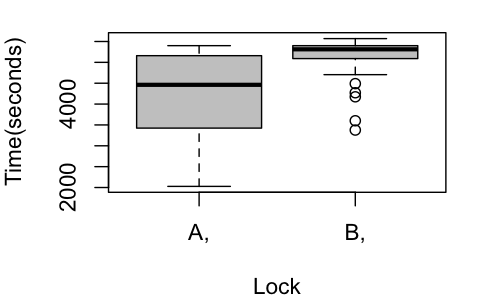
\includegraphics[height=4.5cm]{img/u1.png}
\caption{First experiment box-plot graphic.}\label{fig:boxplot1}
\end{figure}

\begin{table}
\centering
\begin{tabular}{|l|l|l|}
\hline
 & Time Spent (seconds)\\
\hline
LockA & 4227.800 \\
LockB & 5086.367 \\
\hline
\end{tabular}
\caption{First experiment's average time spent}\label{tab:mean1}
\end{table}

Then we run the Box-Cox transformation - a power transformation - to reduce anomalies such as non-additivity and non-normality.
First we verify if the transformation is needed, obtaining the curve in the left of Figure~\ref{fig:transf1}.
Since the value of {\tt lambda} at the maximum point in the curve is not approximately 1, we should apply it.
In order to apply the transformation, $Y_{lijk}$ should be powered to that $\lambda$ on our regression model.
Now, using the transformed model, we obtain the curve shown in the right of Figure~\ref{fig:transf1}.

\begin{figure}
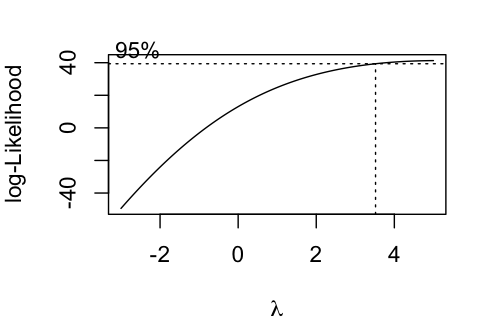
\includegraphics[height=4.5cm, width=6cm]{img/u2.png}
\hfill
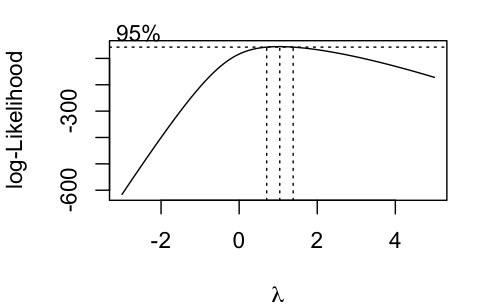
\includegraphics[height=4.3cm, width=6cm]{img/u2boxcox.png}
\caption{First experiment: before and after box-cox transformation ($\lambda = 5$).}\label{fig:transf1}
\end{figure}

In the next step we ran Tukey Test of Additivity to check whether effect model was additive.
Interaction between factors displayed on rows and columns of each latin square won't affect significantly the response only when the model is additive~\cite{box},
so we must verify it (Figure~\ref{tab:tukey}).

\begin{figure}
\centering
\begin{tabular}{ll}
$H_{0}$ & : The model is additive \\
$H_{1}$ & : $H_{0}$ is $false$ \\
\end{tabular}
\caption{Tukey Test of Additivity hypothesis}\label{tab:tukey}
\end{figure}

When the test was executed, we obtained p-value of 0.514, which means we cannot reject $H_{0}$.
Consequently the model was considered to be additive.

Finally, we ran the ANOVA (ANalysis Of VAriance) test which compares the effect of treatments on the response variable,
providing an approximated p-value for every associated factor (see Table~\ref{tab:anova1}).
When a variable has p-value $< 0.05$, it means that factor was statistically significant to the response.
It shows that {\bf lock factor was the most significant to the response}, allowing us to reject our null hypothesis defined in Equation 10.

\begin{table}
\begin{center}
\caption{Undergraduate students experiment ANOVA results.}\label{tab:anova1}
\begin{tabular}{|l|l|l|l|l|ll|}
\hline
                & Df &    Sum Sq  &  Mean Sq   & F value & \emph{p-value} &     \\  
Replica         & 14 & 3.8633e+37 & 2.7595e+36 & 1.6553  & 0.1784197 &     \\   
Program         & 1  & 4.1460e+36 & 4.1460e+36 & 2.4869  & 0.1371197 &     \\   
Lock            & 1  & 3.9489e+37 & 3.9489e+37 & 23.6873 & 0.0002492 & *** \\
Replica:Student & 15 & 4.1013e+37 & 2.7342e+36 & 1.6401  & 0.1808595 &     \\  
Replica:Lock    & 14 & 2.4033e+37 & 1.7166e+36 & 1.0297  & 0.4785520 &     \\  
Residuals       & 14 & 2.3340e+37 & 1.6671e+36 &         &           &     \\
\hline
\end{tabular}
\end{center}
\end{table}

Now we will show the results collected by the second experiment with graduate students. They were exposed to the same set of problems in a different day, but as explained before, they only had a time limit of 1 hour per question.

When we analyze the box-plot for the second group (Image~\ref{fig:boxplot2}) and their average time spent (Table~\ref{tab:mean2}), we can see there was a clear improvement on the time for students using \emph{LockA}.

\begin{figure}
\centering
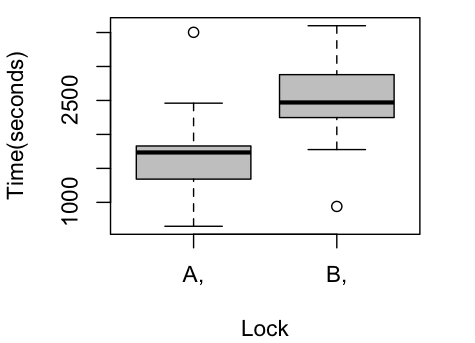
\includegraphics[height=4.5cm]{img/g1.png}
\caption{Second experiment box-plot graphic.}\label{fig:boxplot2}
\end{figure}

\begin{table}
\centering
\begin{tabular}{|l|l|l|}
\hline
 & Time Spent (seconds)\\
\hline
LockA & 1737.714 \\
LockB & 2507.714 \\
\hline
\end{tabular}
\caption{Second experiment's average time spent}\label{tab:mean2}
\end{table}

Moving foward with the analysis, we check if a box-cox transformation is needed. Since the value is not approximately 1, we apply the power transformation the same way we did with the first experiment, but with the corresponding lambda value.

\begin{figure}
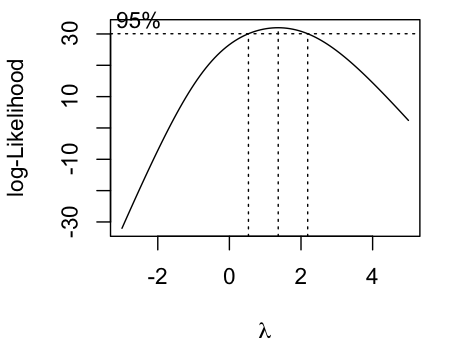
\includegraphics[height=4.5cm]{img/g2.png}
\hfill
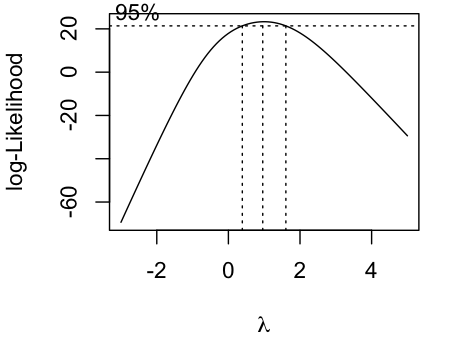
\includegraphics[height=4.4cm]{img/g2boxcox.png}
\caption{Before and after box-cox transformation ($\lambda = 1.3636$).}\label{fig:transf2}
\end{figure}

Finally, running ANOVA, we can see that the type of lock was the most significant factor for the response time, as shown in Table~\ref{tab:anova2}. Again, we can reject the null hypothesis.

\begin{table}
\begin{center}
\caption{Graduate students ANOVA results.}\label{tab:anova2}
\begin{tabular}{|l|l|l|l|l|ll|}
\hline
                 & Df &    Sum Sq &   Mean Sq  & F value &   Pr(>F) & \\   
\hline
replica          & 6 & 2576883250 &  429480542 & 14.1891 & 0.0025793 & **  \\
program          & 1 &    6875586 &    6875586 &  0.2272 & 0.6505035 &     \\
lock             & 1 & 1958179433 & 1958179433 & 64.6938 & 0.0001975 & *** \\
replica:student  & 7 & 2328154077 &  332593440 & 10.9881 & 0.0047601 & **  \\
replica:lock     & 6 &  823830276 &  137305046 &  4.5362 & 0.0441188 & *   \\
Residuals        & 6 &  181610625 &   30268438 &         &           &     \\
\hline
\end{tabular}
\end{center}
\end{table}

\subsubsection{Accuracy Analysis.}

We used the number of correct answers using each lock to measure accuracy, so we defined the following hypothesis to answer {\bf RQ2}. 

\begin{equation}
  H_{0} : \mu_{CorrectAnswersLockA} \leq \mu_{CorrectAnswersLockB}
\end{equation}
\begin{equation}
  H_{1} : \mu_{CorrectAnswersLockA} > \mu_{CorrectAnswersLockB}
\end{equation}

Once we collected all answers, we manually evaluated each one of them according to the criterias established previously, where each criteria had an associated value between 0 and 1. Then we've ran a script that evaluates the equation we defined before to classify whether an answer was correct or not. Grouping the results in tables, we have Table~\ref{tab:acc1} and Table~\ref{tab:acc2}.

\begin{table}
\begin{center}
\caption{Undergraduate students answers accuracy}\label{tab:acc1}
\begin{tabular}{|l|l|l|}
\hline
 & Correct & Incorrect\\
\hline
LockA & 29 & 2\\
LockB & 16 & 15\\
\hline
\end{tabular}
\end{center}
\end{table}

\begin{table}
\begin{center}
\caption{Graduate students answers accuracy}\label{tab:acc2}
\begin{tabular}{|l|l|l|}
\hline
 & Correct & Incorrect\\
\hline
LockA & 13 & 1\\
LockB & 10 & 4\\
\hline
\end{tabular}
\end{center}
\end{table}

Applying Fisher's exact test we can see that undergraduate students results presented a two-tailed P value equals 0.0004: the association between rows (groups) and columns (outcomes) is considered to be extremely statistically significant; consequently, there is clear evidence of improvement on accuracy (see Table~\ref{tab:acc1}).

Meanwhile graduate students results presented a two-tailed P value equals 0.3259, which does not represent a statistically significant evidence of improvement in accuracy (see Table~\ref{tab:acc2}).

% TODO: add script and the data used (anonymized) to appendices or put on github and link %

\subsection{Discussion}

% TODO: review this section, it was written based on older results %

We can see in our results that both groups of students have improved their time to solve the problem when they had the lock with deadlock exception. Also, on the first group, we have found statistically significant evidence that it improved answers accuracy, but not for the second group.

We cannot draw conclusions regarding the improved accuracy on the second group, but we can bring up some relevant aspects we've observed and make a few hypothesis. Some students in the second group were greatly experienced on concurrent programming and they knew how to efficiently find a deadlock using the tools available in Eclipse. Thus, they have finished the exercise really quickly for both problems, knowing exactly which points in the code were involved in the deadlock. So we can see that deadlock exceptions are more helpful for unexperienced programmers in general, and it's possible that even if we had a bigger sample for the second group, we would still not see a significant difference that would indicate deadlock exceptions improved their accuracy.

However, we believe that the benefits of deadlock exceptions are beyond helping unexperienced programmers to find deadlocks more precisely. Experienced programmers would still benefit in many cases where the deadlock is not as obvious as in the exercise we've presented. For example, in a more realistic situation, a deadlock can happen in a background thread that doesn't really affect the program execution overall but make the execution lacking some expected behavior. Furthermore, in non-interactive systems where they are only running in background, is nearly impossible to know when there's a problem unless this software is monitored constantly which is very time consuming or the system produces output constantly that is affected by a potential deadlock. If we have a deadlock exception, we can either prepare and handle this exception on the code level, or just have this signal from output that would help developers to fix it later.

\subsection{Threats To Internal Validity}

In this experiment, we've collected evidence on how the presence of deadlock exception affects student ability to identify deadlocks accurately. However, we must raise a few considerations regarding the validity of our results.

\subsubsection{Time Measurement.}

Since we wanted to run the experiment in a homogenous environment, we've decided to run it in a laboratory in Federal University of Pernambuco, and we've provided links to download the exercise and a few instructions explaining how to deploy it. We wanted to make it as easy as possible and before we've started the test, we gave a small presentation reproducing step by step the instructions that would be described on each exercise, so everyone could follow up and make the setup at the same time. Once everyone was done, we've started to count the time and allowed them to run the programs and start debugging. However, this procedure was not enough: there was a few students (approximately 3 in total) who did the setup differently and could not execute the program; therefore, they've lost a few minutes until we've fixed that for them. Since they've lost only a few minutes, we have still counted them as part of the experiment and did not discount the time.

Furthermore, some students arrived at the test more than 10 minutes late. We've allowed them to join, but some of the remaining computers in the laboratory had issues like they were not logging in or the mouse was not working. We've lost a few minutes to make them work or find a new computer and once each of them did the setup, we've started to count their time individually.

Whenever a student finished a given question, if the time was below the time limit they had available, we have marked the current timestamp on each student's name in the whiteboard. Each entry inserted was already sorted by time, so we easily tracked whether each student was close to the second question's time limit. It would have been better to do this automatically rather than doing manually, so we could potentially reduce overhead of these timestamp operations and increase their precision.

Also, we believe that our imposed time limit have limited more drastically the time ranges on the first group because they spent more time on each question. Also the fact it was an exam for them may have delayed the time to answer because they were more careful. We have observed during the experiment that many students wrote their answers but they were reluctant to ask for the next question because they still have plenty of time left and they wanted to make sure it was correct. We did not observe such behavior with the second group of students and we believe it is because they did not have the same pressure to deliver correct results as the first group had.

\subsubsection{Exercises.}

We understand that the two questions we've used to evaluate the students are far easier than what most software engineers have to deal with in the real world. However we could not use any real world issue because it would easily take the time limit of the experiement for each bug.

On the other hand, we've created two questions based on real world bugs that we have found while searching for deadlock bugs in open source repositories. Each question had a particular level of granularity, where one should be easier to find a bug because of the less amount of code to examine and another that should be more difficult because of the reasonable amount of different files to look at.

Some researchers actually believe that empiric evaluations should not be limited to real projects. Buse claims there are benefits of using non-real artifacts \cite{buse} because it's easier for researchers to translate research questions into successful experiments as it allows a greater control over confouding factors. Otherwise, it would be necessary to turn all participants familiar with the codebase of a real and complex system before even starting the experiment. 

\subsection{Threats to External Validity}

Let's consider a few conditions that might limit the generalization power of our findings in this experiment.

\subsubsection{Students.}

Each student which participated in this experiment had a different background. What we did to minimize the differences was to select groups where students had at least basic experience in concurrent programming and they should be familiarized with the types of bugs such codes can have: the first group of students with undergraduate students attended the class Paradigms of Computaional Languages where deadlocks are covered in classes and exercises; the second group with graduate students attended the class Parallel Programming which covered concurrent programming in low level detail in classes and exercises, including deadlock detection.

Some studies have already addressed the problem of drawing conclusions made with students but some suggest that using students as subjects is as good as using industry professionals \cite{staron}. Runes ran an experiment which shows that there's not much significant differences between undergraduate, graduate and industry professionals, with the exception that undergraduate students often take more time to complete the tasks \cite{runes}.

\subsection{Performance Overhead}\label{sec:perf}

We conducted a preliminary set of experiments to analyze the overhead of our approach.
We compared the our implementation of ReentrantLock with deadlock exceptions, the original ReentrantLock and Eclipse's {\tt OrderedLock}~\cite{orderedlock} implementation in a synthetic benchmark.

OrderedLock is a deadlock-safe implementation of a lock which relies on Eclipse's code architecture.
It is similar our approach in the sense that it attempts to detect deadlocks at runtime. However, it aims to be general, detecting $N$-thread deadlocks without much concern for performance: when a deadlock happens, it releases all locks by a given thread and suspends it, allowing other threads to proceed;
later, the suspended thread will acquire such locks again.
Since it allows threads to temporarily give up all its owned locks, it loses the property of guaranteeing exclusive access policy in \emph{critical zones} that all locks should provide.
In order to use it in our evaluation, as it deeply relies on Eclipse's code architecture to function, we had to perform some small code changes, removing only Eclipse-specific bits that did not affect the core functionality of OrderedLock.
The source code for these lock implementations is available elsewhere~\cite{repo}.

We developed a synthetic benchmark that creates \emph{N} threads that perform additions to ten integer counters where each increment in a counter is protected by explicit locks. Each thread would have to increment its corresponding counter 1000 times before finishing its execution and the counters were evenly distributed across the threads. Therefore, each counter will have exactly \emph{(N / 10)} threads doing increments on it and higher values of \emph{N} result in higher contention, that is, more threads will compete against each other for a particular counter. In this preliminary evaluation, we have conducted measurements for values of $N$ equal to 10, 50, 100, and 200. Since each thread in the benchmark never acquires more than one lock at the same time, deadlocks cannot occur. We emphasize that this setup is very conservative, since every operation that each thread performs requires locking. Thus, the obtained overhead will be a worst-case estimate and thus much higher than one would encounter in a real-world application~\cite{lozi}. The measurements were made on an Intel CoreTM i7 3632QM Processor (6Mb Cache, 2.2GHz) running Ubuntu 12.04.4 LTS and each cell in Table~\ref{tab:overhead} is the average of 50 executions (preceded by 20 executions that served as a warm-up).

\begin{table}
\begin{center}
\caption{Benchmark time measurements (in seconds)}\label{tab:overhead}
\begin{tabular}{|l|l|l|l|}
\hline
\# Threads & ReentrantLock & ReentrantLock Modified & OrderedLock \\
\hline
10 & 0.084184 & 0.105729 & 0.159503\\
50 & 0.089094 & 0.136507 & 1.094718\\
100 & 0.090978 & 0.159541 & 3.395974\\
200 & 0.131739 & 0.194075 & 11.258714\\
\hline
\end{tabular}
\end{center}
\end{table}

The difference of results between our implementation and the original ReentrantLock gives a range of increased time from about 50\% to 90\%. Meanwhile, OrderedLock performed a lot worse, reaching a 8446.3\% increase in time for the worst case. To get a rough estimate of the impact that this overhead would have on actual application execution time, we analyzed the results obtained by Lozi et al.~\cite{lozi}. The authors profiled 19 real-world applications and small benchmarks in order to measure the time these systems spend on their critical sections. Worst-case results ranged between 0.3\% and 92.7\%. If we consider the average time spent on the critical sections of 12 of these systems, the impact of our approach on the overall execution time would be \textbf{less than 6\% in the worst case}. The remaining cases are extreme, in the sense that these systems spend more time in their critical sections than out of them~\cite{lozi}. 




\section{Conclusion}

In this work, we investigated deadlock bug reports in open source projects and
confirmed a previous study claim that TTTL deadlocks
are the most frequent case of deadlock (92.07\% of all resource deadlocks we identified).
We modified Java's \emph{ReentrantLock} and provided a lightweight
version of it that detects TTTL deadlock in runtime.
We measured its performance overhead with a very conservative benchmark
and we estimate our cost to be less than 6\% for worse case on real world applications.
Finally, we did an empirical evaluation to measure its usability and we found that
deadlock exceptions speeds up finding deadlock bugs in code, and we also found some
non-conclusive evidence showing that it may also improve accuracy of deadlock bug reports,
but we leave for future work to verify whether this last observation is actually true.

% References

\begin{references}
  \bibliography{references}
\end{references}

% Appendix

\theappendix
\chapter{Bug Reports Study Attachments}
\label{ap:bug-reports-sample}

\begin{table}[!htp]
	\centering
	\caption{Sampled bug reports (part 1)}
	\label{tbl:conferences_list}
	\rowcolors{2}{lightgray!30}{white}
	\resizebox{\columnwidth}{!}{
	\begin{tabular}{lllll}
	\toprule
	\textbf{BUG} & \textbf{CATEGORY} & \textbf{\# of THREADS} & \textbf{\# of RESOURCES} & \textbf{TYPE} \\
	\toprule
	ECLIPSE-14109  & A        & 2             & 2               & locks/synchronized                          \\
    ECLIPSE-154060 & A        & 2             & 2               & locks/synchronized                          \\
    ECLIPSE-168028 & A        & 2             & 2               & locks/synchronized                          \\
    ECLIPSE-187916 & A        & 2             & 2               & locks/synchronized                          \\
    ECLIPSE-189054 & A        & 2             & 2               & locks/synchronized                          \\
    ECLIPSE-194149 & A        & 2             & 2               & locks/synchronized                          \\
    ECLIPSE-196919 & A        & 2             & 2               & synchronized                                \\
    ECLIPSE-201254 & A        & 2             & 2               & locks/synchronized                          \\
    ECLIPSE-216996 & A        & 2             & 2               & locks/synchronized                          \\
    ECLIPSE-225891 & A        & 2             & 2               & synchronized                                \\
    ECLIPSE-236664 & A        & 2             & 2               & locks/synchronized                          \\
    ECLIPSE-236665 & A        & 2             & 2               & locks/synchronized                          \\
    ECLIPSE-237596 & A        & 2             & 2               & locks/synchronized + static initialization  \\
    ECLIPSE-238304 & A        & 2             & 2               & locks/synchronized                          \\
    ECLIPSE-239309 & A        & 2             & 2               & locks/synchronized                          \\
    ECLIPSE-239672 & A        & 2             & 2               & locks/synchronized                          \\
    ECLIPSE-241713 & A        & 2             & 2               & locks/synchronized                          \\
    ECLIPSE-246284 & A        & 2             & 2               & locks/synchronized                          \\
    ECLIPSE-248908 & A        & 2             & 2               & synchronized                                \\
    ECLIPSE-260777 & A        & 2             & 2               & locks/synchronized                          \\
    ECLIPSE-261476 & A        & 2             & 2               & locks/synchronized                          \\
    ECLIPSE-261664 & A        & 2             & 2               & locks/synchronized                          \\
    ECLIPSE-261910 & A        & 2             & 2               & locks/synchronized                          \\
    ECLIPSE-268572 & A        & 2             & 2               & locks/synchronized                          \\
    ECLIPSE-271840 & A        & 2             & 2               & locks/synchronized                          \\
    ECLIPSE-288945 & A        & 2             & 2               & locks/synchronized                          \\
    ECLIPSE-290550 & A        & 2             & 2               & synchronized                                \\
    ECLIPSE-29212  & A        & 2             & 2               & locks/synchronized                          \\
    ECLIPSE-294913 & A        & 2             & 2               & locks/synchronized                          \\
    ECLIPSE-300596 & A        & 2             & 2               & locks/synchronized                          \\
    ECLIPSE-306219 & A        & 2             & 2               & locks/synchronized                          \\
    ECLIPSE-309781 & A        & 1             & 1               & locks/synchronized                          \\
    ECLIPSE-312504 & A        & 2             & 2               & locks/synchronized                          \\
    ECLIPSE-314176 & A        & 2             & 2               & locks/synchronized                          \\
    ECLIPSE-31891  & A        & 2             & 2               & synchronized                                \\
	\bottomrule
	\end{tabular}
	}
\end{table}

\begin{table}[!htp]
	\centering
	\caption{Sampled bug reports (part 2)}
	\label{tbl:conferences_list}
	\rowcolors{2}{lightgray!30}{white}
	\resizebox{\columnwidth}{!}{
	\begin{tabular}{lllll}
	\toprule
	\textbf{BUG} & \textbf{CATEGORY} & \textbf{\# of THREADS} & \textbf{\# of RESOURCES} & \textbf{TYPE} \\
	\toprule
    ECLIPSE-320182 & A        & 2             & 2               & synchronized                                \\
    ECLIPSE-320760 & A        & 2             & 2               & locks/synchronized                          \\
    ECLIPSE-327247 & A        & 1             & 1               & locks/synchronized                          \\
    ECLIPSE-329302 & A        & 2             & 2               & locks/synchronized                          \\
    ECLIPSE-341849 & A        & 2             & 2               & locks/synchronized                          \\
    ECLIPSE-343012 & A        & 2             & 2               & locks/synchronized                          \\
    ECLIPSE-347183 & A        & 1             & 1               & locks                                       \\
    ECLIPSE-358396 & A        & 3             & 2               & locks/synchronized                          \\
    ECLIPSE-359580 & A        & 2             & 2               & locks/synchronized + static initialization  \\
    ECLIPSE-359698 & A        & 2             & 2               & locks/synchronized                          \\
    ECLIPSE-359851 & A        & 2             & 2               & locks/synchronized                          \\
    ECLIPSE-361533 & A        & 2             & 2               & locks/synchronied + static initialization   \\
    ECLIPSE-374272 & A        & 3             & 1               & locks/synchronized                          \\
    ECLIPSE-375601 & A        & 2             & 2               & locks/synchronized                          \\
    ECLIPSE-381580 & A        & 2             & 2               & locks/synchronized                          \\
    ECLIPSE-384204 & A        & 2             & 2               & locks/synchronized                          \\
    ECLIPSE-389630 & A        & 2             & 2               & locks/synchronized                          \\
    ECLIPSE-390963 & A        & 3             & 2               & locks/synchronized                          \\
    ECLIPSE-39104  & A        & 2             & 2               & locks/synchronized                          \\
    ECLIPSE-393277 & A        & 2             & 2               & locks/synchronized                          \\
    ECLIPSE-395211 & A        & 2             & 2               & locks/synchronized                          \\
    ECLIPSE-397442 & A        & 3             & 2               & locks/synchronized                          \\
    ECLIPSE-40114  & A        & 2             & 2               & locks/synchronized                          \\
    ECLIPSE-405511 & A        & 2             & 2               & locks/synchronized + output stream          \\
    ECLIPSE-407513 & A        & 2             & 2               & locks/synchronized                          \\
    ECLIPSE-413730 & A        & 2             & 2               & locks/synchronized                          \\
    ECLIPSE-416088 & A        & 2             & 2               & locks/synchronized                          \\
    ECLIPSE-428335 & A        & 2             & 2               & locks/synchronized                          \\
    ECLIPSE-47647  & A        & 2             & 2               & locks/synchronized                          \\
    ECLIPSE-49708  & A        & 2             & 2               & locks/synchronized                          \\
    ECLIPSE-50949  & A        & 2             & 2               & synchronized                                \\
    ECLIPSE-58892  & A        & 2             & 2               & synchronized                                \\
    ECLIPSE-60856  & A        & 2             & 2               & locks/synchronized                          \\
    ECLIPSE-61179  & A        & 2             & 2               & locks/synchronized                          \\
    ECLIPSE-62398  & A        & 2             & 2               & locks/synchronized                          \\
    ECLIPSE-67181  & A        & 2             & 2               & locks/synchronized                          \\
    ECLIPSE-70557  & A        & 2             & 2               & locks/synchronized                          \\
    ECLIPSE-75115  & A        & 2             & 2               & locks/synchronized                          \\
    ECLIPSE-79394  & A        & 2             & 2               & locks/synchronized                          \\
    ECLIPSE-80610  & A        & 2             & 2               & locks/synchronized                          \\
    ECLIPSE-86614  & A        & 2             & 2               & locks/synchronized                          \\
    JDK-4101618    & A        & 2             & 2               & locks/synchronized                          \\
    JDK-4192666    & A        & 2             & 2               & locks/synchronized                          \\
    JDK-4258193    & A        & 2             & 2               & locks/synchronized                          \\
    JDK-4265501    & A        & 2             & 2               & locks/synchronized                          \\
    JDK-4294865    & A        & 2             & 2               & locks/synchronized                          \\
    JDK-4826573    & A        & 2             & 2               & locks/synchronized                          \\
    JDK-4828019    & A        & 2             & 2               & locks/synchronized                          \\
    JDK-4852569    & A        & 2             & 2               & locks/synchronized                          \\
    JDK-4944382    & A        & 2             & 2               & locks/synchronized                          \\
    JDK-4965227    & A        & 2             & 2               & locks/synchronized                          \\
    JDK-5006427    & A        & 2             & 2               & locks/synchronized                          \\
	\bottomrule
	\end{tabular}
	}
\end{table}

\begin{table}[!htp]
	\centering
	\caption{Sampled bug reports (part 3)}
	\label{tbl:conferences_list}
	\rowcolors{2}{lightgray!30}{white}
	\resizebox{\columnwidth}{!}{
	\begin{tabular}{lllll}
	\toprule
	\textbf{BUG} & \textbf{CATEGORY} & \textbf{\# of THREADS} & \textbf{\# of RESOURCES} & \textbf{TYPE} \\
	\toprule
    JDK-6190373    & A        & 2             & 2               & locks/synchronized                          \\
    JDK-6296324    & A        & 2             & 2               & locks/synchronized                          \\
    JDK-6349844    & A        & 2             & 2               & locks/synchronized                          \\
    JDK-6362921    & A        & 2             & 2               & locks/synchronized                          \\
    JDK-6370241    & A        & 4             & 4               & locks/synchronized                          \\
    JDK-6373352    & A        & 2             & 2               & locks/synchronized                          \\
    JDK-6440846    & A        & 2             & 2               & locks/synchronized                          \\
    JDK-6814140    & A        & 2             & 2               & locks/synchronized                          \\
    JDK-6834576    & A        & 2             & 2               & locks/synchronized                          \\
    JDK-8026356    & A        & 2             & 2               & locks/synchronized                          \\
    LUCENE-1200    & A        & 2             & 2               & synchronized                                \\
    LUCENE-1358    & A        & 2             & 2               & synchronized                                \\
    LUCENE-2783    & A        & 2             & 2               & locks/synchronized                          \\
    LUCENE-3705    & A        & 2             & 2               & lock + synchronized                         \\
    ECLIPSE-188320 & B        & ~             & ~               & wait/notify                                 \\
    ECLIPSE-199565 & B        & 2             & ~               & synchronized + notify/signal                \\
    ECLIPSE-199568 & B        & 2             & ~               & synchronized + notify/signal                \\
    ECLIPSE-220452 & B        & 2             & 1               & synchronized + join                         \\
    ECLIPSE-226376 & B        & 2             & 1               & synchronized + join                         \\
    ECLIPSE-283490 & B        & ~             & ~               & wait + message                              \\
    ECLIPSE-295796 & B        & ~             & ~               & wait/notify                                 \\
    ECLIPSE-296570 & B        & ~             & ~               & wait/notify                                 \\
    ECLIPSE-305611 & B        & ~             & ~               & locks/synchronized + notify                 \\
    ECLIPSE-311863 & B        & ~             & ~               & wait/notify                                 \\
    ECLIPSE-323680 & B        & 2             & 2               & synchronized + wait                         \\
    ECLIPSE-330937 & B        & 2             & 1               & synchronized + wait                         \\
    ECLIPSE-341196 & B        & 2             & ~               & wait/notify                                 \\
    ECLIPSE-357278 & B        & 2             & 1               & synchronized + wait                         \\
    ECLIPSE-362238 & B        & 2             & 1               & locks/synchronized + wait                   \\
    ECLIPSE-362288 & B        & ~             & ~               & wait/notify                                 \\
    ECLIPSE-385921 & B        & ~             & ~               & locks/synchronized + join                   \\
    ECLIPSE-391046 & B        & 2             & 1               & locks/synchronized                          \\
    ECLIPSE-411029 & B        & 2             & ~               & ~                                           \\
    ECLIPSE-426785 & B        & 2             & ~               & ~                                           \\
    ECLIPSE-52859  & B        & ~             & ~               & wait/notify                                 \\
    ECLIPSE-53466  & B        & ~             & ~               & wait/notify                                 \\
    ECLIPSE-71382  & B        & 2             & ~               & wait                                        \\
    JDK-4529917    & B        & ~             & ~               & wait/notify                                 \\
    JDK-4636269    & B        & ~             & ~               & wait/notify                                 \\
    JDK-4760364    & B        & 2             & ~               & wait/notify                                 \\
    JDK-4962516    & B        & ~             & ~               & wait/notify                                 \\
    JDK-6253009    & B        & 2             & 1               & lock + wait                                 \\
    LUCENE-1544    & B        & 2             & ~               & ~                                           \\
    LUCENE-3528    & B        & ~             & ~               & wait/notify                                 \\
    LUCENE-4071    & B        & ~             & ~               & wait/notify                                 \\
    LUCENE-5002    & B        & 2             & 1               & synchronized + wait/notify                  \\
	\bottomrule
	\end{tabular}
	}
\end{table}

\begin{table}[!htp]
	\centering
	\caption{Sampled bug reports (part 4)}
	\label{tbl:conferences_list}
	\rowcolors{2}{lightgray!30}{white}
	\resizebox{\columnwidth}{!}{
	\begin{tabular}{lllll}
	\toprule
	\textbf{BUG} & \textbf{CATEGORY} & \textbf{\# of THREADS} & \textbf{\# of RESOURCES} & \textbf{TYPE} \\
	\toprule
    ECLIPSE-148367 & C        & ~             & ~               & ~                                           \\
    ECLIPSE-164848 & C        & ~             & ~               & ~                                           \\
    ECLIPSE-168034 & C        & ~             & ~               & ~                                           \\
    ECLIPSE-186783 & C        & ~             & ~               & ~                                           \\
    ECLIPSE-223154 & C        & ~             & ~               & ~                                           \\
    ECLIPSE-231274 & C        & ~             & ~               & ~                                           \\
    ECLIPSE-234452 & C        & ~             & ~               & ~                                           \\
    ECLIPSE-234916 & C        & ~             & ~               & ~                                           \\
    ECLIPSE-246795 & C        & ~             & ~               & ~                                           \\
    ECLIPSE-246983 & C        & ~             & ~               & ~                                           \\
    ECLIPSE-249085 & C        & ~             & ~               & ~                                           \\
    ECLIPSE-261667 & C        & ~             & ~               & ~                                           \\
    ECLIPSE-328082 & C        & ~             & ~               & ~                                           \\
    ECLIPSE-361541 & C        & ~             & ~               & ~                                           \\
    ECLIPSE-43202  & C        & ~             & ~               & ~                                           \\
    JDK-4352221    & C        & ~             & ~               & ~                                           \\
    JDK-6225372    & C        & ~             & ~               & ~                                           \\
    JDK-6381164    & C        & ~             & ~               & ~                                           \\
    LUCENE-1210    & C        & ~             & ~               & ~                                           \\
    LUCENE-2095    & C        & ~             & ~               & ~                                           \\
    LUCENE-2216    & C        & ~             & ~               & ~                                           \\
    LUCENE-2820    & C        & ~             & ~               & ~                                           \\
    LUCENE-3348    & C        & ~             & ~               & ~                                           \\
    ECLIPSE-101944 & D        & ~             & ~               & ~                                           \\
    ECLIPSE-122144 & D        & ~             & ~               & ~                                           \\
    ECLIPSE-150198 & D        & ~             & ~               & ~                                           \\
    ECLIPSE-196290 & D        & ~             & ~               & locks/synchronized                          \\
    ECLIPSE-203306 & D        & ~             & ~               & ~                                           \\
    ECLIPSE-212617 & D        & ~             & ~               & ~                                           \\
    ECLIPSE-218145 & D        & ~             & ~               & ~                                           \\
    ECLIPSE-236259 & D        & ~             & ~               & ~                                           \\
    ECLIPSE-243450 & D        & ~             & ~               & ~                                           \\
    ECLIPSE-246151 & D        & ~             & ~               & ~                                           \\
    ECLIPSE-259143 & D        & ~             & ~               & ~                                           \\
    ECLIPSE-263689 & D        & ~             & ~               & ~                                           \\
    ECLIPSE-26540  & D        & ~             & ~               & ~                                           \\
    ECLIPSE-267801 & D        & ~             & ~               & ~                                           \\
    ECLIPSE-270762 & D        & ~             & ~               & ~                                           \\
    ECLIPSE-282188 & D        & ~             & ~               & ~                                           \\
    ECLIPSE-289122 & D        & ~             & ~               & ~                                           \\
    ECLIPSE-289553 & D        & ~             & ~               & ~                                           \\
    ECLIPSE-291877 & D        & 2             & ~               & ~                                           \\
    ECLIPSE-296056 & D        & 2             & ~               & ~                                           \\
    ECLIPSE-299184 & D        & ~             & ~               & ~                                           \\
    ECLIPSE-300451 & D        & ~             & ~               & locks/synchronized + wait?                  \\
    ECLIPSE-30140  & D        & ~             & ~               & ~                                           \\
    ECLIPSE-303670 & D        & ~             & ~               & ~                                           \\
    ECLIPSE-306914 & D        & ~             & ~               & ~                                           \\
    ECLIPSE-308120 & D        & ~             & ~               & ~                                           \\
    ECLIPSE-310007 & D        & ~             & ~               & ~                                           \\
	\bottomrule
	\end{tabular}
	}
\end{table}

\begin{table}[!htp]
	\centering
	\caption{Sampled bug reports (part 5)}
	\label{tbl:conferences_list}
	\rowcolors{2}{lightgray!30}{white}
	\resizebox{\columnwidth}{!}{
	\begin{tabular}{lllll}
	\toprule
	\textbf{BUG} & \textbf{CATEGORY} & \textbf{\# of THREADS} & \textbf{\# of RESOURCES} & \textbf{TYPE} \\
	\toprule
	ECLIPSE-314923 & D        & ~             & ~               & ~                                           \\
    ECLIPSE-319168 & D        & ~             & ~               & ~                                           \\
    ECLIPSE-326274 & D        & ~             & ~               & ~                                           \\
    ECLIPSE-327472 & D        & ~             & ~               & ~                                           \\
    ECLIPSE-328697 & D        & ~             & ~               & ~                                           \\
    ECLIPSE-330505 & D        & 2             & ~               & ~                                           \\
    ECLIPSE-330964 & D        & ~             & ~               & ~                                           \\
    ECLIPSE-335235 & D        & ~             & ~               & ~                                           \\
    ECLIPSE-338965 & D        & ~             & ~               & ~                                           \\
    ECLIPSE-348284 & D        & ~             & ~               & ~                                           \\
    ECLIPSE-359199 & D        & ~             & ~               & ~                                           \\
    ECLIPSE-361302 & D        & 2             & 1               & locks/synchronized + wait?                  \\
    ECLIPSE-366784 & D        & ~             & ~               & ~                                           \\
    ECLIPSE-37614  & D        & ~             & ~               & ~                                           \\
    ECLIPSE-390600 & D        & ~             & ~               & ~                                           \\
    ECLIPSE-42096  & D        & ~             & ~               & ~                                           \\
    ECLIPSE-428937 & D        & ~             & ~               & ~                                           \\
    ECLIPSE-434645 & D        & ~             & ~               & ~                                           \\
    ECLIPSE-43571  & D        & ~             & ~               & ~                                           \\
    ECLIPSE-4365   & D        & ~             & ~               & ~                                           \\
    ECLIPSE-50639  & D        & ~             & ~               & ~                                           \\
    ECLIPSE-59816  & D        & ~             & ~               & ~                                           \\
    ECLIPSE-83415  & D        & ~             & ~               & ~                                           \\
    JDK-4176738    & D        & ~             & ~               & ~                                           \\
    JDK-4366691    & D        & ~             & ~               & ~                                           \\
    JDK-4646297    & D        & ~             & ~               & ~                                           \\
    JDK-4762958    & D        & ~             & ~               & ~                                           \\
    JDK-4881251    & D        & ~             & ~               & ~                                           \\
    JDK-5083318    & D        & 2             & ~               & ~                                           \\
    JDK-5106770    & D        & ~             & ~               & ~                                           \\
    JDK-6303187    & D        & ~             & ~               & ~                                           \\
    JDK-6377483    & D        & ~             & ~               & ~                                           \\
    JDK-6386537    & D        & ~             & ~               & ~                                           \\
    JDK-6899078    & D        & ~             & ~               & ~                                           \\
    JDK-6949705    & D        & ~             & ~               & ~                                           \\
    JDK-7100952    & D        & ~             & ~               & ~                                           \\
    JDK-7105040    & D        & ~             & ~               & ~                                           \\
    JDK-7171163    & D        & ~             & ~               & ~                                           \\
    JDK-7174887    & D        & ~             & ~               & ~                                           \\
    LUCENE-1171    & D        & ~             & ~               & ~                                           \\
    LUCENE-159     & D        & ~             & ~               & ~                                           \\
    LUCENE-4147    & D        & ~             & ~               & ~                                           \\
	\bottomrule
	\end{tabular}
	}
\end{table}
\begin{table}[!htp]
	\centering
	\caption{Bug report study: search queries and results}
	\label{tab:bug-reports-queries}
	\rowcolors{2}{lightgray!30}{white}
	\resizebox{\columnwidth}{!}{
	\begin{tabular}{lll}
	\toprule
	Project & Query Parameters                                                                           & Results URL          \\
	\toprule
    Lucene  & lucene-core, bug, status:"closed", assignee:all, "deadlock"                                & http://goo.gl/DhVI3t \\
    Eclipse & summary:"deadlock", resolution:"fixed", status:"resolved"                                  & http://goo.gl/qQnrEm \\
    OpenJDK & project:"JDK", summary:"deadlock", issue type:"bug", status:"resolved", resolution:"fixed" & http://goo.gl/xYFfsO \\
    \hline
    Sampled & & http://goo.gl/zNsIGz \\
	\bottomrule
	\end{tabular}
	}
\end{table}


\chapter{Evaluation Chapter Attachments}
\label{ap:evaluation-instructions}

\section{Time Analysis}

\medskip
\noindent
{\it R Instructions}
\begin{verbatim}
exp1.dat = read.table(file="/home/me/r_input.dat", header = T)
attach(exp1.dat)

replica = factor(replica.)
student = factor(student.)
program = factor(program.)
lock = factor(lock.)

# Calculate average time for each lock

aggregate(time, by=list(lock), FUN=mean)

# Plot the box plot graphic using the response variable
# associated with the techniques

plot(time~lock,col="gray",xlab="Lock",ylab="Time(seconds)")

# Through the following command we adjust the effect model
# that will serve as basis for posterior analysis.

anova.ql<-aov(time~replica+student:replica+program+lock)

library(MASS)
bc <- boxcox(anova.ql,lambda = seq(-3, 5, 1/10))

# Calculate lambda for boxcox transformation

lambda <- bc$x[which.max(bc$y)] 

# If lambda is not approximately 1, run the next command
# with [a] replaced by lambda's value found previously:
# anova.ql<-aov(time**[a]~replica+student:replica+program+lock)
# Then confirm that the new curve maximum is close to 1: 
# bc <- boxcox(anova.ql,lambda = seq(-3, 5, 1/10))

TukeyNADD.QL.REP<-function(objeto1)
{
y1<-NULL
y2<-NULL
y1<- fitted(objeto1)
y2<- y1^2
objeto2<- aov(y2 ~ objeto1[13]$model[,2] +
objeto1[13]$model[,3]:objeto1[13]$model[,2]
+ objeto1[13]$model[,4]+ objeto1[13]$model[,5])
ynew <- resid(objeto1)
xnew <- resid(objeto2)
objeto3 <- lm(ynew ~ xnew)
M <- anova(objeto3)
MSN <- M[1,3]
MSErr <- M[2,2]/(objeto1[8]$df.residual-1)

F0 <- MSN/MSErr
p.val <- 1 - pf(F0, 1,objeto1[8]$df.residual-1)
p.val
}

# Return p-value for Tukey additivity test
TukeyNADD.QL.REP(anova.ql)

# Run ANOVA to see what factor was most significant
anova(anova.ql)
\end{verbatim}

\medskip
\noindent
{\it First Experiment Input}
\begin{verbatim}
replica, student, program, lock, time
1, 1, p1, A, 4967
1, 1, p2, B, 5413
1, 2, p1, B, 5400
1, 2, p2, A, 5320
2, 3, p1, A, 2340
2, 3, p2, B, 5290
2, 4, p1, B, 5400
2, 4, p2, A, 4210
3, 5, p1, A, 5400
3, 5, p2, B, 5360
3, 6, p1, B, 3600
3, 6, p2, A, 2406
4, 7, p1, A, 3290
4, 7, p2, B, 5370
4, 8, p1, B, 5070
4, 8, p2, A, 5260
5, 9, p1, A, 3000
5, 9, p2, B, 5315
5, 10, p1, B, 5400
5, 10, p2, A, 3641
6, 11, p1, A, 3424
6, 11, p2, B, 5356
6, 12, p1, B, 5400
6, 12, p2, A, 4788
7, 13, p1, A, 5400
7, 13, p2, B, 5400
7, 14, p1, B, 5400
7, 14, p2, A, 5160
8, 15, p1, A, 5280
8, 15, p2, B, 5160
8, 16, p1, B, 4490
8, 16, p2, A, 4017
9, 17, p1, A, 2700
9, 17, p2, B, 5306
9, 18, p1, B, 5090
9, 18, p2, A, 4450
10, 19, p1, A, 4271
10, 19, p2, B, 5569
10, 20, p1, B, 3377
10, 20, p2, A, 4473
11, 21, p1, A, 5160
11, 21, p2, B, 5430
11, 22, p1, B, 4174
11, 22, p2, A, 4886
12, 23, p1, A, 2027
12, 23, p2, B, 4271
12, 24, p1, B, 5400
12, 24, p2, A, 3804
13, 25, p1, A, 4996
13, 25, p2, B, 5367
13, 26, p1, B, 5310
13, 26, p2, A, 5390
14, 27, p1, A, 3860
14, 27, p2, B, 5119
14, 28, p1, B, 4705
14, 28, p2, A, 4535
15, 29, p1, A, 2593
15, 29, p2, B, 5279
15, 30, p1, B, 5250
15, 30, p2, A, 4246
\end{verbatim}

\medskip
\noindent
{\it Second Experiment Input}
\begin{verbatim}
replica, student, program, lock, time
1, 1, p1, A, 1757
1, 1, p2, B, 2404
1, 2, p1, B, 1777
1, 2, p2, A, 1716
2, 3, p1, A, 1342
2, 3, p2, B, 2552
2, 4, p1, B, 2597
2, 4, p2, A, 1238
3, 5, p1, A, 1572
3, 5, p2, B, 2248
3, 6, p1, B, 3168
3, 6, p2, A, 2460
4, 7, p1, A, 1822
4, 7, p2, B, 2455
4, 8, p1, B, 2486
4, 8, p2, A, 2434
5, 9, p1, A, 3503
5, 9, p2, B, 3600
5, 10, p1, B, 2454
5, 10, p2, A, 1753
6, 11, p1, A, 1830
6, 11, p2, B, 3300
6, 12, p1, B, 2880
6, 12, p2, A, 890
7, 13, p1, A, 648
7, 13, p2, B, 940
7, 14, p1, B, 2247
7, 14, p2, A, 1363
\end{verbatim}

\section{Accuracy Analysis}

\medskip
\noindent
{\it R Instructions}
\begin{verbatim}
# Use TSV export feature on each set of results:
# [1] https://goo.gl/EPxmEa (first experiment)
# [2] https://goo.gl/rsWPwi (second experiment)
# Run http://pastebin.com/rSBjTiYj on each

fisher.test(rbind(c(29,2),c(16,15)), alternative="two.sided")
fisher.test(rbind(c(13,1),c(10,4)), alternative="two.sided")
\end{verbatim}

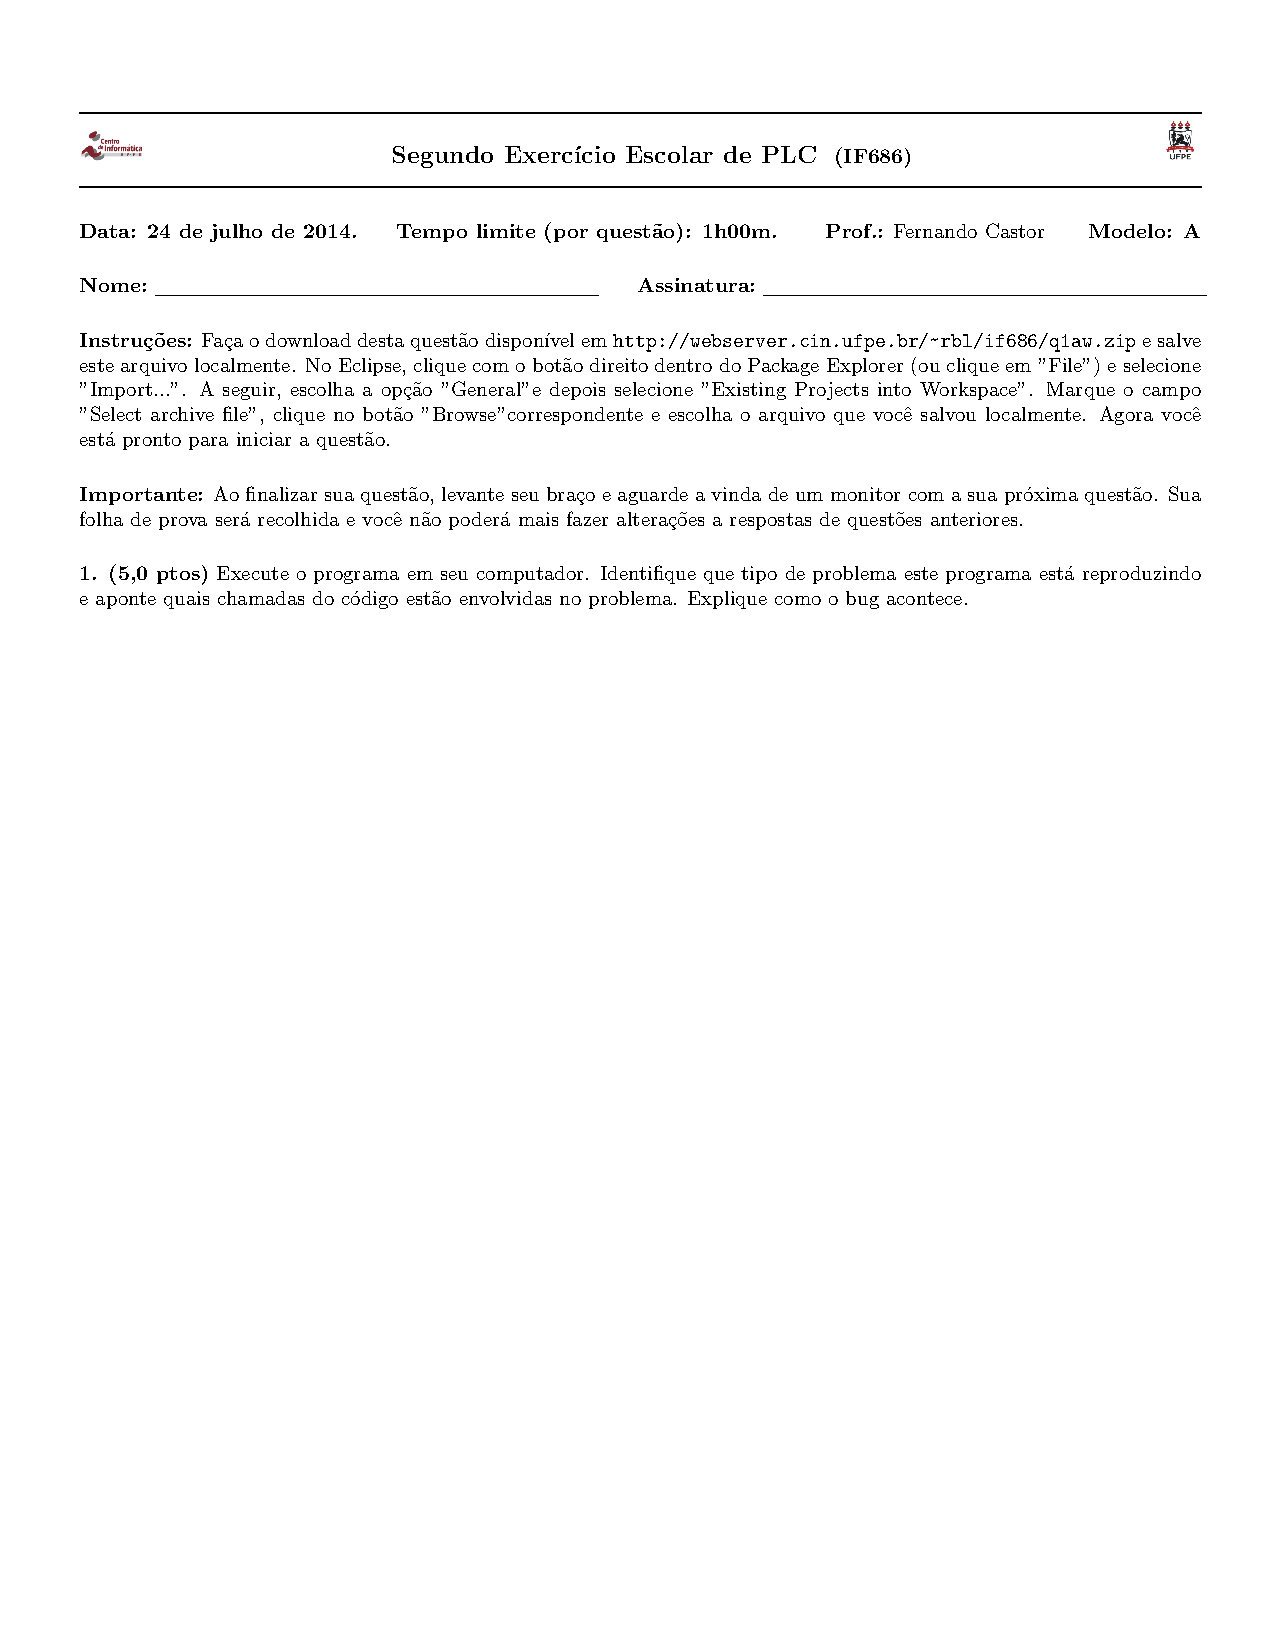
\includepdf[scale=0.8,pages=1,pagecommand=\section{Experiment First Assignment}]{appendix/sample-question.pdf}

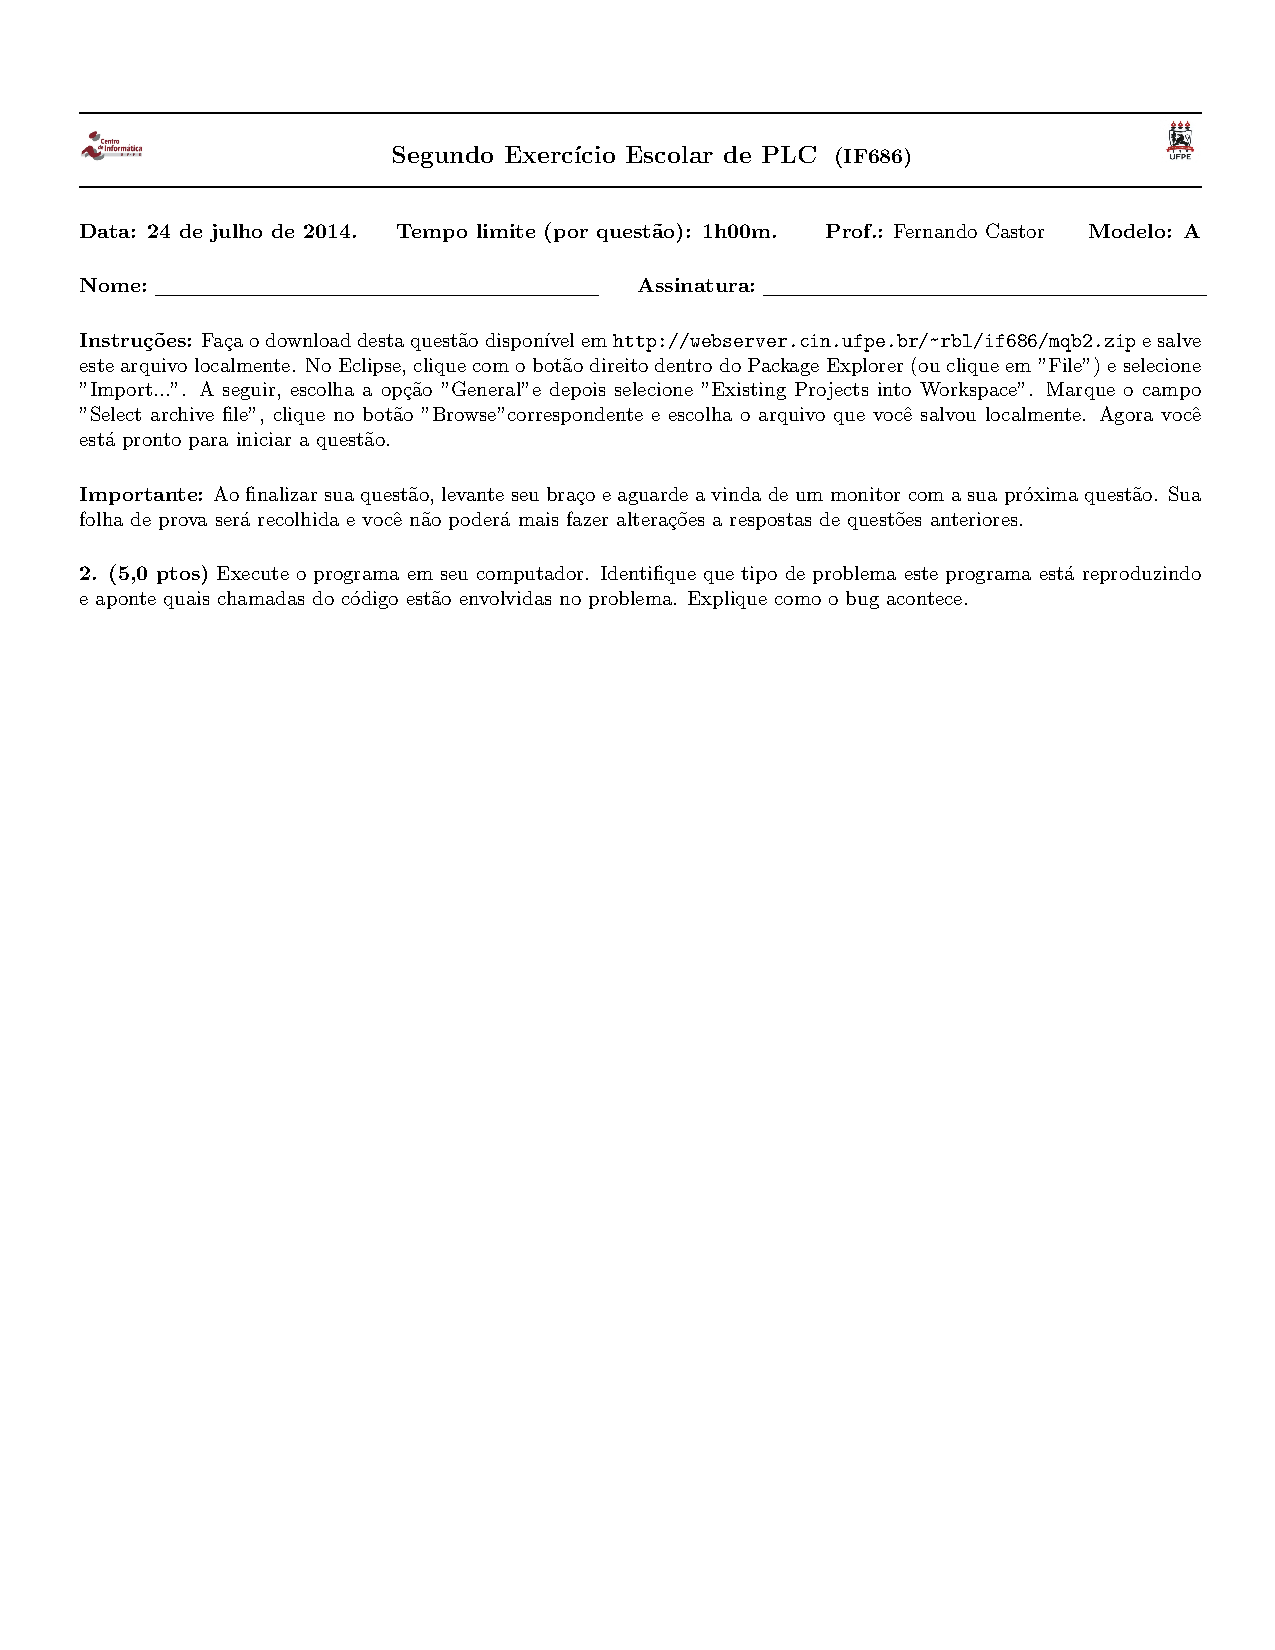
\includepdf[scale=0.8,pages=1,pagecommand=\section{Experiment Second Assignment}]{appendix/sample-question-2.pdf}



\end{document}
